\documentclass[11pt,oneside]{book}
%%%%%%%%%%%%%%%%%%%%%%%%%%%%%%%%%%%%%%%%%%%%%%%%%%%%%
% [topsep=0pt,itemsep=-1ex,partopsep=1ex,parsep=1ex]%
%%%%%%%%%%%%%%%%%%%%%%%%%%%%%%%%%%%%%%%%%%%%%%%%%%%%%
%%%%%%%%%%%%%%Include Packages%%%%%%%%%%%%%%%%%%%%%%%%%%
\usepackage[legalpaper, margin=1in]{geometry}
\usepackage[dvipsnames]{xcolor}
\usepackage{mathtools}
\usepackage{amsmath}
\usepackage{amssymb}
\usepackage{rsfso}
\usepackage{amsthm}
\usepackage{wasysym}
\usepackage[inline]{enumitem}   
\usepackage{hyperref}
\usepackage{tocloft}
\usepackage{titlesec}
\usepackage{colortbl}
\usepackage{stackengine}
\usepackage{afterpage}
%%%%%%%%%%%%%%%%%%%%%%%%%%%%%%%%%%%%%%%%%%%%%%%%%%%%%%%%


%%%%%%%%%%%%%%%Chapter Setting%%%%%%%%%%%%%%%%%%%%%%%%%%
\definecolor{gray75}{gray}{0.75}
\newcommand{\hsp}{\hspace{20pt}}
\titleformat{\chapter}[hang]{\Huge\bfseries}{\thechapter\hsp\textcolor{gray75}{$\mid$}\hsp}{0pt}{\Huge\bfseries}
%%%%%%%%%%%%%%%%%%%%%%%%%%%%%%%%%%%%%%%%%%%%%%%%%%%%%%%%

%%%%%%%%%%%%%%%%%Theorem environments%%%%%%%%%%%%%%%%%%%
\newtheoremstyle{break}
  {\topsep}{\topsep}%
  {\itshape}{}%
  {\bfseries}{}%
  {\newline}{}%
\theoremstyle{break}
\theoremstyle{break}
\newtheorem{axiom}{Axiom}
\newtheorem{thm}{Theorem}[section]
\renewcommand{\thethm}{\arabic{section}.\arabic{thm}}
\newtheorem{lem}{Lemma}[thm]
\newtheorem{prop}[lem]{Proposition}
\newtheorem{corL}{Corollary}[lem]
\newtheorem{corT}[lem]{Corollary}
\newtheorem{defn}{Definition}[corL]
\newenvironment{indEnv}[1][Proof]
  {\proof[#1]\leftskip=1cm\rightskip=1cm}
  {\endproof}
%%%%%%%%%%%%%%%%%%%%%%%%%%%%%%%%%%%%%%%%%%%%%%%%%%%%%%

%%%%%%%%%%%%%%%%%%%%%%%Integral%%%%%%%%%%%%%%%%%%%%%%%
\def\upint{\mathchoice%
    {\mkern13mu\overline{\vphantom{\intop}\mkern7mu}\mkern-20mu}%
    {\mkern7mu\overline{\vphantom{\intop}\mkern7mu}\mkern-14mu}%
    {\mkern7mu\overline{\vphantom{\intop}\mkern7mu}\mkern-14mu}%
    {\mkern7mu\overline{\vphantom{\intop}\mkern7mu}\mkern-14mu}%
  \int}
\def\lowint{\mkern3mu\underline{\vphantom{\intop}\mkern7mu}\mkern-10mu\int}
%%%%%%%%%%%%%%%%%%%%%%%%%%%%%%%%%%%%%%%%%%%%%%%%%%%%%%



\newcommand{\R}{\mathbb{R}}
\newcommand{\N}{\mathbb{N}}
\newcommand{\Z}{\mathbb{Z}}
\newcommand{\Q}{\mathbb{Q}}
\newcommand{\D}{\mathcal{D}}
\newcommand{\J}{\mathcal{J}}
\newcommand{\T}{\mathcal{T}}
\newcommand{\C}{\mathcal{C}}
\newcommand{\M}{\mathcal{M}}
\newcommand{\X}{x}
\newcommand{\Lt}{\mathcal{L}}
\newcommand{\A}{\mathcal{A}}
\newcommand{\Complex}{\mathbb{C}}
\newcommand{\Power}{\mathcal{P}}
\newcommand{\Symm}{\text{Symm}}
\newcommand{\Alt}{\text{Alt}}
\newcommand{\Int}{\text{Int}}
\newcommand{\spa}{\text{span}}
\newcommand{\supp}{\text{supp}}
\newcommand{\sgn}{\text{sgn}}
\newcommand{\degr}{\text{deg}}
\newcommand{\Bd}{\text{Bd}}
\newcommand{\ee}{\cdot 10}
\newcommand{\pd}{\partial}
\newcommand{\that}[1]{\widetilde{#1}}
\newcommand{\lr}[1]{\left(#1\right)}
\newcommand{\vmat}[1]{\begin{vmatrix} #1 \end{vmatrix}}
\newcommand{\bmat}[1]{\begin{bmatrix} #1 \end{bmatrix}}
\newcommand{\pmat}[1]{\begin{pmatrix} #1 \end{pmatrix}}
\newcommand{\rref}{\xrightarrow{\text{row\ reduce}}}
\newcommand{\txtarrow}[1]{\xrightarrow{\text{#1}}}
\newcommand\oast{\stackMath\mathbin{\stackinset{c}{0ex}{c}{0ex}{\ast}{\Circle}}}
\newcommand*{\Perm}[2]{{}^{#1}\!P_{#2}}
\newcommand*{\Comb}[2]{{}^{#1}C_{#2}}

\newcommand{\note}{\color{Purple}Note: \color{black}}
\newcommand{\remark}{\color{blue}Remark: \color{black}}
\newcommand{\example}{\color{WildStrawberry}Example: \color{black}}
\newcommand{\exercise}{\color{CadetBlue}Exercise: \color{black}}

%%%%%%%%%%%%%%%%%%%%%%Roman Number%%%%%%%%%%%%%%%%%%%%%%%
\makeatletter
\newcommand*{\rom}[1]{\expandafter\@slowromancap\romannumeral #1@}
\makeatother
%%%%%%%%%%%%%%%%%%%%%%%%%%%%%%%%%%%%%%%%%%%%%%%%%%%%%%%%%

%%%%%%%%%%%%table of contents%%%%%%%%%%%%%%%%%%%%%%%%%%%%
\setlength{\cftchapindent}{0em}
\setlength{\cftsecindent}{2em}
\renewcommand\cfttoctitlefont{\hfill\huge\bfseries}
\renewcommand\cftaftertoctitle{\hfill\mbox{}}
\setcounter{tocdepth}{2}
%%%%%%%%%%%%%%%%%%%%%%%%%%%%%%%%%%%%%%%%%%%%%%%%%%%%%%%%%


%%%%%%%%%%%%%%%%%%%%%Footnotes%%%%%%%%%%%%%%%%%%%%%%%%%%%
\newcommand\blfootnote[1]{%
  \begingroup
  \renewcommand\thefootnote{}\footnote{#1}%
  \addtocounter{footnote}{-1}%
  \endgroup
}
%%%%%%%%%%%%%%%%%%%%%%%%%%%%%%%%%%%%%%%%%%%%%%%%%%%%%%%%%

%%%%%%%%%%%%%%%%%%%Hide Section Number%%%%%%%%%%%%%%%%%%%
\makeatletter
\def\@seccntformat#1{%
  \expandafter\ifx\csname c@#1\endcsname\c@section\else
  \csname the#1\endcsname\quad
  \fi}
\makeatother
%%%%%%%%%%%%%%%%%%%%%%%%%%%%%%%%%%%%%%%%%%%%%%%%%%%%%%%%%

%%%%%%%%%%%%%%%%%%%%%%%%%%%%%%%%%%%Enumerate%%%%%%%%%%%%%
\makeatletter
% This command ignores the optional argument 
% for itemize and enumerate lists
\newcommand{\inlineitem}[1][]{%
\ifnum\enit@type=\tw@
    {\descriptionlabel{#1}}
  \hspace{\labelsep}%
\else
  \ifnum\enit@type=\z@
       \refstepcounter{\@listctr}\fi
    \quad\@itemlabel\hspace{\labelsep}%
\fi}
\makeatother
\parindent=0pt
%%%%%%%%%%%%%%%%%%%%%%%%%%%%%%%%%%%%%%%%%%%%%%%%%%%%%%%%%

\definecolor{DarkBlue}{RGB}{19,15,50}


\begin{document}
%	\pagecolor{DarkBlue}
	\begin{titlepage}
		\begin{center}
			\topskip0pt
			\vspace*{\fill}
			\Huge \color{red}
				\textbf{Class Notes}\\
				\color{black}
			\vspace{0.5cm}			
			\Large 
				STAT410 - Introduction to Probability Theory\\
				Professor Jonathan Francis Fernandes\\
				University of Maryland, College Park
			\vspace{3cm}

			
			
			\vspace{5cm}
			\LARGE
				\textbf{Wenyu Chen}\\
				\hfill\break
				\LARGE Summer 2022\\
				\color{black}
			\vspace{5cm}

		\vspace*{\fill}
		\author{Wenyu Chen} \date{Summer 2022}
		\end{center}			
%		\afterpage{\nopagecolor}
	\end{titlepage}
	\newpage
	\tableofcontents
	\newpage
	\chapter[Axioms of Probabilities]{\color{WildStrawberry}Axioms of Probabilities\color{black}}
	\section[Basic Definition of Probabilities]{Basic Definition of Probabilities}
	\begin{defn}
	\textbf{Experiment:} is repeatable task with well defined outcomes.\\
	\textbf{Sample Space:} is a collection of all possible outcomes of the experiment.\\
	\textbf{Event:} is a subset of the sample space.
	\end{defn}
	\hfill\\
	\example Suppose we toss a coin three times, assume coins lands on H or T.\\
	\textbf{Experiment: }tossing the coin three times, noting the outcomes.\\
	\textbf{Sample Space:} $\{$HHH, HHT,HTH, THH, HTT,THT,TTH, TTT $\}$\\
	\textbf{Example of events:} $E_1=$ getting all heads $=\{HHH\}\subseteq S$\\ 
	$E_2=$ getting exactly one H and one T $=\{\}\subseteq S$\\
	$E_3=$ getting at least two heads $=\{HHH, HHT, HTH, THH\}\subseteq S$\\
	\hfill\\
	We want to assign a number to each event, which is a measure of the chance or probabilities that this event happened. Our goal is to understand the process of assigning probabilities to events.\\
	\hfill\\
	\example \textbf{Die Roll}\\
	\textbf{Experiment:} Roll a six sided dice two times\\
	\textbf{Sample Space:}$\{(1,1),(1,2)...(1,6),(2,1)...(2,6)...(6,6)\}$\\
	\textbf{Example of events:} \\
	$E_1=$ at least one six = $\{(1,6),(2,6),(3,6),(4,6),(5,6),(6,6),(6,1),(6,2),(6,3),(6,4),(6,5)\}$\\
	$|E_2|=10$\\
	$E_2=$ same numbers on both rolls = $\{(1,1),(2,2),(3,3),(4,4),(5,5),(6,6)\}$\\
	$E_4=\{(1,5),(3,4)\}$\\
	\hfill\\
	\note\\ 
	\textbf{Simple Event:} is the event with exactly one outcomes. It is the cardinality of the sample space. \\
	\textbf{Number of events:} Assume the sample space is finite of size n, the number of events is the cardinality of all possible outcomes of S $=2^n$\\
	\hfill\\
	\textbf{Set in context}\\
	Let an event E be describes as a subset of the sample space S.\\
	Let E, F two events be given.\\
	$E\cap F$ is a new event that corresponds to outcomes in both E and F\\
	$E\cup F$ is a outcome a new event include outcomes in E or F\\
	$E^c$ is a new event that include outcomes where E doesn't happen.\\
	\hfill\\
	When we say an event E has happened, we means that the outcome $\omega$ of the experiment lies inside E\\
	\example Tossed a coin three times. In one run of the experiment, the result is HHT.\\
	HHT $\in E_1=$ at least two heads, we said $E_1$ has happened.\\
	\begin{defn}
	A sigma algebra $\mathcal{B}$ for a set S is a collection of subset of S that satisfies:\begin{enumerate}
	\item $\emptyset \in \mathcal{B}$
	\item If $A\in \mathcal{B}$ then $A^c\in \mathcal{B}$ (closed under complement)
	\item If $\{A_i\}_{i=1}^{\infty} \in \mathcal{B}$ then $\bigcup_{i=1}^{\infty} A_i \in \mathcal{B}$ (closed under countable unions)
	\end{enumerate}
	\end{defn}
	\note 	Sigma algebra is a collection of events to which we want to assign the probabilities.\\
	\example Recall back to the dice roll example. Let B be the power set of its sample space. Then
note it is the sigma algebra of the sample space. The size will be $2^{|s|} = 236$\\
\example: Let event E of S be given. Then its sigma algebra $B = \{\emptyset,E,E^c, S\}$
	\section[Axioms for a probability function]{\color{Periwinkle}Axioms for a probability function\color{black}}
	\begin{defn}
Suppose we are given the pair $(S,\mathcal{B})$, where S represents the sample space and $\mathcal{B}$ is a sigma algebra S. 
	A \textbf{probability function} P satisfies the following:\begin{align*}
	P:\mathcal{B}\rightarrow \mathbb{R}\\
	E \mapsto P(E)
	\end{align*}
	\begin{enumerate}
	\item $P(A)\geq 0$ for all $A\in \mathcal{B}$
	\item $P(S)=1$
	\item If $A_1,A_2,A_3,...$ are mutually disjiont sets in $\mathcal{B}$ then $P\lr{\bigcup_{i=1}^{\infty}A_i}=\sum_{i=1}^{\infty}P(A_i)$
	\end{enumerate}
	\end{defn}
	\begin{thm}
	\textbf{Properties of a probability function:} Suppose $P:\mathcal{B}\rightarrow \mathbb{R}$ is a probability function. Then\begin{enumerate}
	\item $P(\emptyset)=0$
	\item $P(A)\leq 1$ for all $A\in \mathcal{B}$
	\item $P(A^c)=1-P(A)$
	\item $P(A\cap B^c)=P(A)-P(A\cap B)$
	\item $P(A\cup B)=P(A)+P(B)-P(A\cap B)$
	\end{enumerate}
	\end{thm}
	\begin{thm}
	Suppose the sample space S is countable. To define a probability function on $(S,\mathcal{B}=P(S))$, we do the following \begin{enumerate}
	\item Find a seq $\{p_i\}_{i=1}^{\infty}$ such that (i) $0\leq p_i\leq 1, \forall i$ and (ii) $\sum_{i=1}^{\infty}p_i=1$
	\item Define $P(\{s_i\})=p_i$
	\item For any $E\in \mathcal{B}, E=\{s_{i1},s_{i2},...s_{ik}\}$ \begin{align*}
		 P(E)=\sum_{j=1}^{k}P(S_{ij})=\sum_{j=1}^{k}P_{ij}
		 \end{align*}
	\end{enumerate}
	\end{thm}
	\example Probability Functions Examples\\
\text{\quad} Coin Tosseo: \\
\text{\quad} \textbf{Experiment: }tossing the coin three times, noting the outcomes.\\
\text{\quad} \textbf{Sample Space:} $\{$HHH, HHT,HTH, THH, HTT,THT,TTH, TTT $\}$\\
	To get a probability function, we will need to work with a sigma algebra. Suppose $\mathcal{B}_1=\mathcal{P}(S)$, note that the cardinality of $\mathcal{B}_1$ is 256.\\
	There are infinitely many ways to choose the sequence ${p_i}$. One way is to choose $p_i=\frac{1}{8}$ for all i. Then we assign the probability.\\
\begin{center}
\begin{tabular}{|l|l|l|l|l|l|l|l|l|}
\hline
$S_i$    & HHH           & HHT           & HTH           & THH           & HTT           & THT           & TTH           & TTT           \\ \hline
$P(S_i)$ & $\frac{1}{8}$ & $\frac{1}{8}$ & $\frac{1}{8}$ & $\frac{1}{8}$ & $\frac{1}{8}$ & $\frac{1}{8}$ & $\frac{1}{8}$ & $\frac{1}{8}$ \\ \hline
\end{tabular}
\end{center}
It is clear that the third properties is satisfied. For example, if $E=\{HHT, HTH, TTT\}$, then \begin{align*}
P(E)&= P(HHT)+P(HTH)+P(TTT)\\
&= \frac{1}{8}+\frac{1}{8}+\frac{1}{8}\\
&=\frac{3}{8}
\end{align*}
	 Another way is to set $p_1=1$ and rest to 0. Then, we got \begin{center}
\begin{tabular}{|l|l|l|l|l|l|l|l|l|}
\hline
$S_i$    & HHH & HHT & HTH & THH & HTT & THT & TTH & TTT \\ \hline
$P(S_i)$ & 1   & 0   & 0   & 0   & 0   & 0   & 0   & 0   \\ \hline
\end{tabular}
 \end{center}
 It is clear that the third properties is satisfied. For example, if $E=\{HHT, HTH, TTT\}$, then \begin{align*}
P(E)&= P(HHT)+P(HTH)+P(TTT)\\
&= 0 + 0 + 0 \\
&= 0
\end{align*}

	Alternate way to assign probabilities is to use the information about the experiment, and need to construct tree diagrams. 
	\textbf{Tree Diagram} is a graph that describes the flow of the outcomes of each steps in an experiment. 
	\begin{defn}
	\textbf{Conditional Probability} is $P(A\mid B)$= P(A happens given that B has already happened)\begin{align*}
	=\frac{P(A\cap B)}{P(B)}
	\end{align*}
	And by \textbf{Multiplication Principle}, \begin{align*}
	P(A\cap B) & = P(A\mid B) \times P(B)\\
	&= P(B\mid A)\times P(A)
	\end{align*}
	\end{defn}
	\textbf{Experiment:} Toss a fixed coin three times. We need to know that $P(H)=p\in (0,1)$. Then we can got the tree diagram as\\
	\hfill\\
	 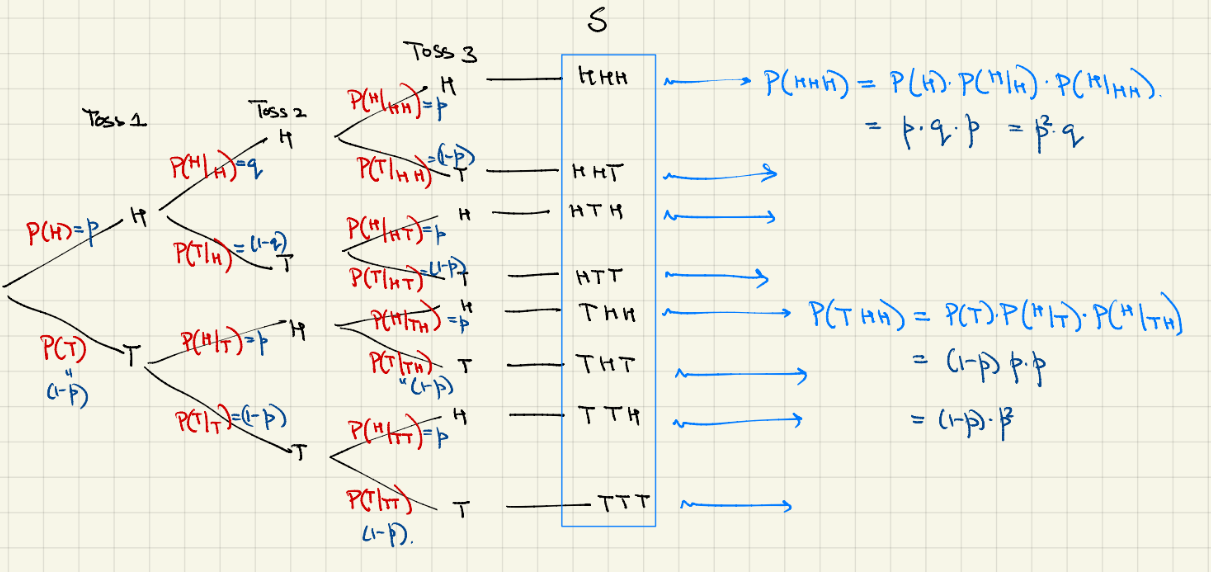
\includegraphics[scale=0.35]{figures/graph}\\
	 Then we can just assign p in (0,1). Then the rest can be assigned through the tree diagram.\\
\hfill\\
\hfill\\
	Assumption: 1) Probability of events when all outcomes in the sample space are equally likely. 2) Sample space is finite.
	\begin{prop}
	If every outcome in the sample space is equally likely, we can calculate the probability of $E\subseteq S$ as follow: \begin{align*}
	P(E)=\frac{n(E)}{n(S)}
	\end{align*}
	where $n(E)$ is the number of outcomes in E. 
	\end{prop}
	\example Suppose we toss a coin that $p(H)\in (0,1)$ two times. The sample space is S = $\{$HH, HT, TH, TT$\}$. If the coin is fair, then $P(HH)=P(HT)=P(TH)=P(TT)=0.25$\\
	\hfill\\
	\begin{thm}
	\textbf{Fundmental Theorem of Counting:} Suppose a task T can be performed as a sequence of subtasks: $T_1,T_2,T_3,...,T_k$. And each $n_1,...,n_2,n_3,...,n_k$ is number of ways to perform $T_i$\\
	Then the total number ways to perform the task T is  \begin{align*}
	n_1\times n_2 \times n_3 \times \cdots \times n_k
	\end{align*}
	\end{thm} 
	Typically we will have to select k objects from n distinct objects.\\
	\example $\{0,1,2,3,4,5,6,7,8,9\}$, we might be interested in knowing the total number of ways one can choose 4 digits from this 10 digits.\\
	\hfill\\
\begin{tabular}{l|l|l|}
\cline{2-3}
                                                                                       & Without Replacement                                                                                    & With Replacement                                                                                   \\ \hline
\multicolumn{1}{|l|}{Order Matters}                                                    & \begin{tabular}[c]{@{}l@{}}(1,2,4,5) different from (1,5,2,4)\\ (1,1,2,5) is not possible\end{tabular} & \begin{tabular}[c]{@{}l@{}}(1,2,4,5) different from (1,5,2,4)\\ (1,1,2,5) is possible\end{tabular} \\ \hline
\multicolumn{1}{|l|}{\begin{tabular}[c]{@{}l@{}}Order Does Not\\ Matters\end{tabular}} & \begin{tabular}[c]{@{}l@{}}(1,2,3,4) is same as (4,3,2,1)\\ (1,1,2,5) not possible\end{tabular}        & \begin{tabular}[c]{@{}l@{}}(1,2,3,4) is same as (4,3,2,1)\\ (1,1,2,4) is possible\end{tabular}     \\ \hline
\end{tabular}\\
\hfill\\
\hfill\\
\textbf{1. Without replacement and order matters}\\
Use the fundamental theorem of counting, we divide T, which is select k digits from a set of n distinct objects divide into \begin{align*}
T:T_1\rightarrow T_2\rightarrow T_3 \rightarrow \cdots \rightarrow T_k
\end{align*}
where $T_i$ is select ith object. Then, we will got \begin{align*}
n\times (n-1)\times (n-2) \times (n-3) \times \cdots \times (n-k+1)
\end{align*}
Then, we got \begin{align*}
\Perm{n}{k}=\frac{n!}{(n-k)!}
\end{align*}
\hfill\\
\textbf{2. Without replacement and order does not matter}\\
T = choose k objects from n distinct objects where order does not matter and without replacement. \begin{align*}
T:T_1\rightarrow T_2
\end{align*}
$T_1$ is choose k objects where order matters and without replacement \\
$T_2$ is to get rid of all the times we have double counted.\\
\hfill\\
$\#$ ways to do $T_1=\Perm{n}{k}=\frac{n!}{(n-k)!}$\\
$\#$ ways to do $T_2=$ number of arrangements of k objects $=k!$\\
Then we got \begin{align*}
\Comb{n}{k}=\binom nk =\frac{n!}{(n-k)!k!}
\end{align*}
\textbf{3. With replacement and order does not matter}\\
$T=$ Choose k objects where order does not matter and with replacement. \\
\hfill\\
We keep track of how many times a given object repeats in the selection and the total number of objects in the selection is equal to k. To do so, we can have $n+k-1$ spots with n-1 walls (since it is with replacement) as following\begin{center}
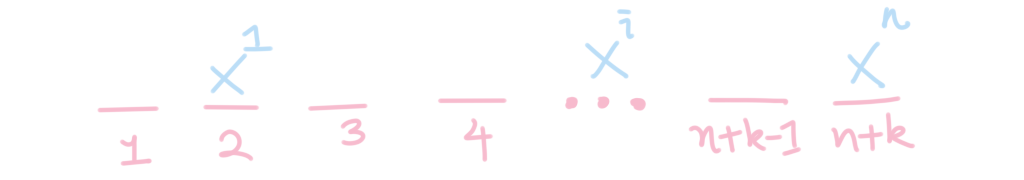
\includegraphics[scale=0.3]{figures/withreplacement_doesnt_matter}
\end{center}
Notice that the $x^{n}$ wall is always in the last place, so we only need to consider a length of $n+k-1$. And the space left represents number of objects in this set. By placing the wall differently, we will get different combination of objects with a total number of k. \\
\hfill\\
So we need to decide from $n+k-1$ spots to determine which are the $n-1$ walls. Notice that the order doesn't matter and we don't have replacement. Therefore, we got
 \begin{align*}
\Comb{n+k-1}{k}=\Comb{n+k-1}{n-1}
\end{align*}
\hfill\\
\example $\{1,2,3,4\}$, $k=10$, We are selecting 10 objects from $\{1,2,3,4\}$ with replacement and order does not matter.\\
We only care about how many times each number shows up since order does not matter and the total objects in selection are 10. To achieve that, we setup 13 spots. Such that, the extra position is the walls.\\
\hfill\\
\textbf{4.With Replacement}\\
Choose k objects where order does matter and with replacement in n different things is \begin{align*}
n^k
\end{align*}
\chapter[Conditional Probability, Independence, and Bayes' Theorem]{ \color{WildStrawberry} Conditional Probability, Independence, and Bayes' Theorem \color{Black}}
Recall: Given two events A and B, the conditional probability is \begin{align*}
P(A\mid B)=\frac{P(A\cap B)}{P(B)}
\end{align*}
as long as $P(B)>0$\\
\hfill\\
And \textbf{Multiplication Principle} is \begin{align*}
P(A\cap B)&=P(A\mid B)\cdot P(B)\\
&=P(B\mid A)\cdot P(A)\\
\end{align*}
\begin{defn}
We say two events A and B are \textbf{independent} if and only if \begin{align*}
P(A\cap B)&=P(A)\cdot P(B)
\end{align*}
which is equivalent to saying that fact B occured does not affect the probability of A happening.\begin{align*}
P(A\mid B)&=P(A)
\end{align*}
and equivalent to saying that the fact A occurred does not affect the probability of B happening\begin{align*}
P(B\mid A)&=P(B)
\end{align*}
\end{defn}
\hfill\\
\example 
Now if A and B are independent can show that A and $B^c$ are also independent.\\
\textbf{Hint:} note that $P(A\cap B^c)$ can be write in term of $P(A),P(B),P(A\cap B)$
\begin{proof}
\begin{align*}
(A\cap B^c)&=P(A)+P(B^c)-P(A\cup B^c)\\
&=P(A)+P(B^c)-P(B^c\cup (A\cap B))\\
&=P(A)+P(B^c)-(P(B^c)+ (A\cap B))\\
&=P(A)+P(B^c)-P(B^c)- (A\cap B))\\
&=P(A)-(A\cap B))\\
&=P(A)-P(A)\cdot P(B)\\
&=P(A)(1-P(B))\\
&=P(A)\cdot P(B^c)
\end{align*}
\end{proof}
\begin{thm}
\textbf{The Law of Total Probability} \\
If $A_1,A_2, A_3,...,A_k$ is a partition of the sample space S, meaning
\begin{center} 
(i) $A_i's$ are mutually disjoint (ii) $\bigcup_{i=1}^{k}=S$
\end{center}
Then for any event B in the sigma algebra associate with S\begin{align*}
P(B)&=P(B\cap S)=P\left(B\cap \left(\bigcup_{i=1}^{k}A_i\right)\right)\\
&=\sum_{i=1}^{k}P(B\cap A_i)\\
&=P(B\cap A_1)+P(B\cap A_2)+\cdots +P(B\cap A_k)
\end{align*}
\end{thm}
Visually, \begin{center}
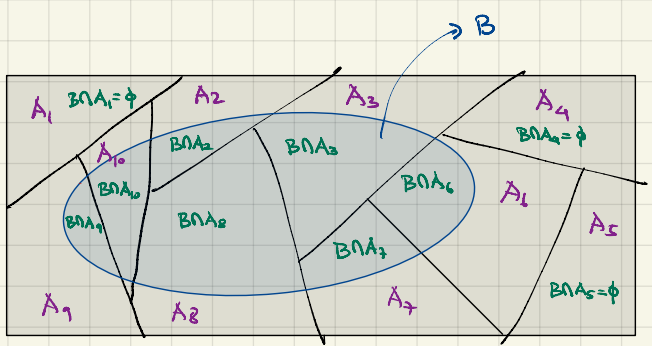
\includegraphics[scale=0.9]{figures/visual_total_law}
\end{center}
\begin{thm}
\textbf{Bayes' Theorem}: \\
If $A_1,A_2, A_3,...,A_k$ is a partition of the sample space S, then for any event B in sigma algebra associated with S, and for any i, \begin{align*}
P(A_i\mid B)&=\frac{P(A_i\cap B)}{P(B)} &\text{by multiplication of principle}\\
&=\frac{P(A_i\cap B)}{\sum_{j=1}^{k}P(A_j\cap B)} &\text{using the law of total probability}\\
&=\frac{P(B\mid A_i)\cdot P(A_i)}{\sum_{j=1}^{k}P(B\mid A_j)\cdot P(A_j)} &\text{by multiplication of principle}\\
\end{align*}
\end{thm}
\example Assume there is an experiment\\
\text{\qquad} \textbf{Step 1:} Toss a coin with P(H)=0.4\\
\text{\qquad} \textbf{Step 2:} If H in step 1, roll a fair die.\\
\text{\qquad} \text{\qquad} \text{\quad} If T in step 1, we roll an unfair die with $P(1)=P(2)=\cdots=P(5)=0.1$ and $P(6)=0.5$\\
\hfill\\
 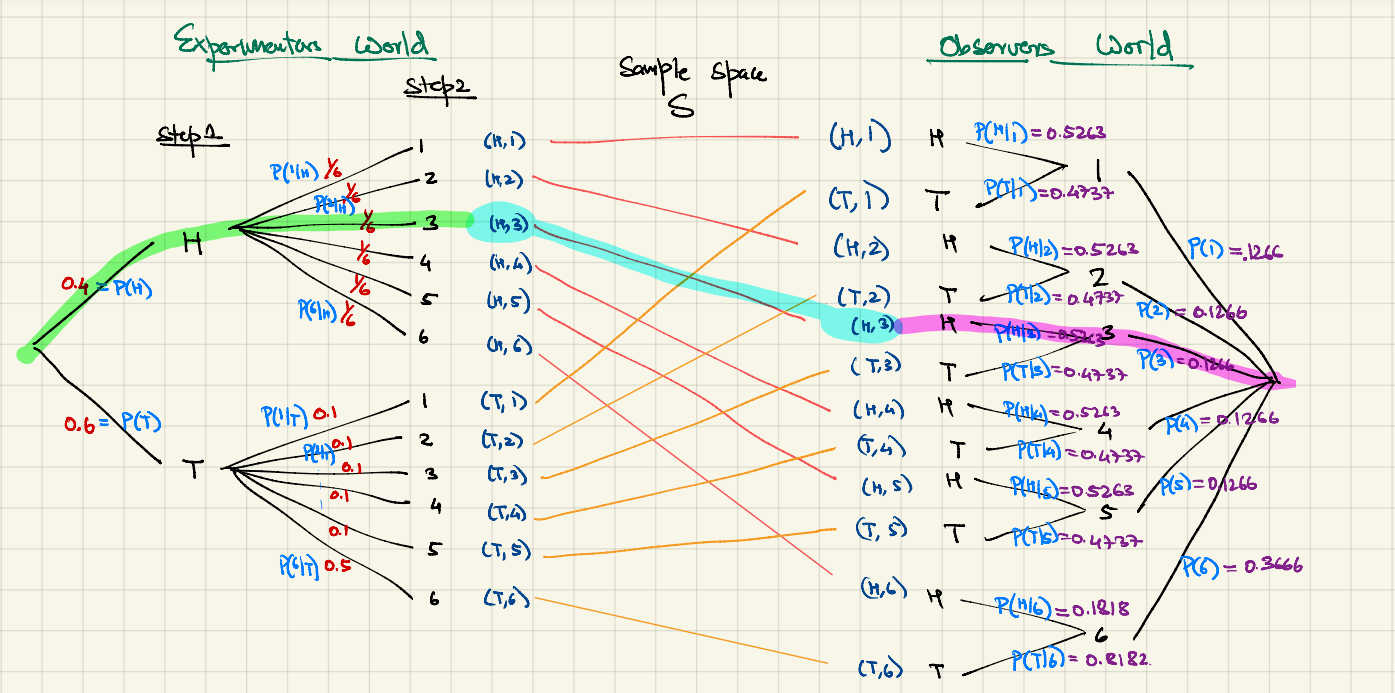
\includegraphics[scale=0.7]{figures/example2}\\
 If an observer see a 6, then \begin{align*}
 P(H\mid 6)&=\frac{P(H,6)}{P(6)}=\frac{P(H,6)}{P(H,6)+P(T,6)}\\
 &=\frac{0.4\times \frac{1}{6}}{0.4\times \frac{1}{6}+0.6*0.5}\\
 &=0.1818
 \end{align*}
\newpage
\chapter[Random Variables]{Random Variables}
\section[Introduction to Random Variable]{Introduction to Random Variable}
\begin{defn}
A \textbf{random variable} is a function defined on a sample space S such that \begin{align*}
X:S\rightarrow \mathbb{R}\\
\omega \mapsto X(\omega) \in \mathbb{R}
\end{align*}
\end{defn}
\begin{defn}
Given X, we consider the set \begin{center}
X := values of the random variable X.
\end{center}
For $x\in \mathbb{R}$, we define \begin{align*}
\{X=x\}&:=\{\omega\in S\mid X(w)=x\}\\
&=X^{-1}(x)
\end{align*}
Also, \begin{align*}
\{X\leq x\}&:=\{\omega \in S \mid X(\omega)\leq x\}
\end{align*}
and for $a,b\in \mathbb{R}$\begin{align*}
\{a\leq x\leq b\}
\end{align*}
and for $a,b\in \mathbb{R}$\begin{align*}
\{a\leq X\leq b\}&:=\{\omega\in S\mid a\leq X(\omega)\leq b\}\\
&=X^{-1}([a,b])
\end{align*}
\end{defn}
\example \textbf{Experiment:} Toss a voin three times\\
\text{\qquad} \text{\qquad} \textbf{Sample Space:} $\{$TTT, TTH, THT, HTT, THH, HTH, HHT, HHH$\}$\\
Now given an outcome in S, want to attach a number. Then we define a random variable X \begin{align*}
X:S&\rightarrow \mathbb{R}\\
\omega &\mapsto X(\omega)= \text{ number of H in }\omega\\
X&=\{0,1,2,3\}
\end{align*}
Then \begin{align*}
\{x=0\}&=\{TTT\}\\
\{x=1\}&=\{HTT,THT,TTH\}\\
\{x=2\}&=\{HHT,HTH,THH\}\\
\{x=3\}&=\{HHH\}
\end{align*}
Then, we can define a probability function for the pair $(S,\mathcal{B})$ where the sigma algebra is generated by $<\{x=0\},\{x=1\},\{x=2\},\{x=3\}>$. Here is the distribution table for P defined for the pair $(S,\mathcal{B})$ \begin{center}
\begin{tabular}{|l|l|l|l|l|}
\hline
x        & 0             & 1             & 2             & 3             \\ \hline
$P(X=\mathcal{X})$ & $\frac{1}{8}$ & $\frac{3}{8}$ & $\frac{3}{8}$ & $\frac{1}{8}$ \\ \hline
\end{tabular}
\end{center}
Also, the distribution table for $(S,\mathcal{B}(\mathcal{P}(S)))$ is  \begin{center}
\begin{tabular}{|l|l|l|l|l|l|l|l|l|}
\hline
 $\omega$& TTT & TTH & THT & HTT & THH & HTH & HHT & HHH \\ \hline
 $P(\omega)$&  $\frac{1}{8}$   &   $\frac{1}{8}$   &    $\frac{1}{8}$  &   $\frac{1}{8}$   &   $\frac{1}{8}$   &   $\frac{1}{8}$   &   $\frac{1}{8}$   &  $\frac{1}{8}$    \\ \hline
\end{tabular}
\end{center}
The advantages of using first distribution table is 1) has less columns than the second distribution table, which makes visualizing and analyzing substantial easier. 2) It combines information that is relevant to the question we interested in. 3) X is a new sample space subset of $\mathcal{R}$ so we can use the properties of $\mathcal{R}$\\
\begin{defn}
\textbf{Induced Probability Function:}\\
Suppose we have a probability function P defined on $(S,\mathcal{P}(S))$. Then, if X is a random variable with values $x$, we can define\begin{align*}
P_X(\{X=x\})&:=\sum_{\omega\in \{X=x\}}P(\omega)
\end{align*}
And for any subset $E\subseteq x$\begin{align*}
P_X(E)&=P_X\left( \bigcup_{x\in E}\{X=x\}\right)\\
&=\sum_{x\in E}P(\{X=x\})
\end{align*}
\end{defn}
\begin{defn}
\textbf{The Cummulative Distribution Function of X}\\
Given a random variable $X:S\rightarrow \mathbb{R}$, the cumulative distribution function, is defined as :\begin{align*}
F_X:\mathbb{R}\rightarrow \mathbb{R}\\
F_X(x):=P(X\leq x)
\end{align*}
\end{defn}
\begin{defn}
We say two random variables X and Y are identically distributed if they have the same cumulative distribution function, i.e\begin{align*}
F_X(u)=F_y(u) \text{\qquad} \forall u\in \mathbb{R}
\end{align*}
\end{defn}
\example Back to the previous example with X is the number of heads in the toss, we can get
\begin{center}
 $F_X(x)= \begin{cases}
0 & x<0\\
\frac{1}{8} & x\in [0,1)\\
\frac{4}{8} & x\in [1,2)\\
\frac{7}{8} & x\in [1,2)\\
1 & x\in [3,\infty)
\end{cases}$
\end{center}
And the graph of $F_X(x)$\begin{center}
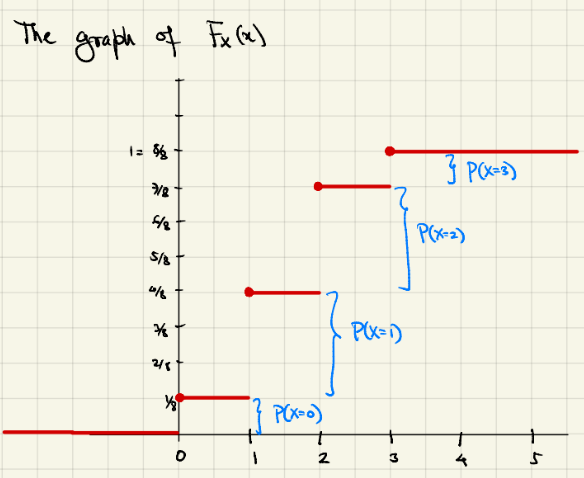
\includegraphics[scale=0.5]{figures/graph_example}
\end{center}
\note We say $X$ is discrete if $F_X$ is a step function.\\
\text{\quad}\text{\qquad}We say $X$ is continuous if $F_X$ is continuous function.\\
\begin{thm}
\textbf{Classification of Cumulative Distribution Function For Random Variables}\\
The $F(x)$ is a cumulative distribution function of a random variable if and only if the following condition hold \begin{enumerate}
\item $\lim_{x\rightarrow \infty}F(x)=1$ and $\lim_{x\rightarrow -\infty}F(x)=0$ is right continuous
\item $F(x)$ is a non-decreasing function
\item $F(x)$ is right continuous
\end{enumerate}
\end{thm}
\note Random Variable X can be discrete, continuous, or neither discrete nor continuous.
\section[Expected Values, Variance, Moment Generating Function]{Expected Values, Variance, Moment Generating Function}
\begin{defn}
\textbf{Expected Value} of a random variable X is longterm average value X will take if experiment is performed repeatedly.  
\end{defn}
\begin{defn}
\textbf{Variance} is expected squared deviation of the values of X from its expected value. \\
If the variance small, it will be more confident.
\end{defn}
\begin{thm}
Suppose X is a \textbf{discrete} random variable, meaning the cumulative distribution function $F_X(x)$ is a step function. \\
The \textbf{Probability Mass Function} of X is \begin{align*}
p_X(\X)&:=P(X=\X)\text{\qquad} \X\in \mathbb{R}
\end{align*}
The \textbf{Expected Values} of X is \begin{align*}
M_X&:=E(X):=\sum_{\X\in X}\X \cdot p_X(\X)
\end{align*}
if $h:\R\rightarrow \R$ is any function, then\begin{align*}
E(h(X))&=\sum_{\X\in X}h(\X)p_X(\X)
\end{align*}
The \textbf{Variance} of X is \begin{align*}
V(X)&:=\sigma_X^2=E((X-M_X)^2)\\
&=\sum_{\X\in X}(\X-M_X)^2p_X(\X)
\end{align*}
The \textbf{Moment Generating Function }of X is \begin{align*}
M_X(t)&=E(e^{tx}):=\sum_{\X\in X}e^{t\X}\cdot p_X(\X)
\end{align*}
\end{thm}
\begin{thm}
Suppose X is a \textbf{continuous} random variable, meaning the cummulative distribution function $F_X(\X)$ is continuous.\\
The \textbf{Probability Density Function} for X, a function $f_X:\R \rightarrow \R$ satisfies the following \begin{align*}
F_X(\X)&=P(X\leq \X)=\int_{-\infty}^{\X}f_X(t)dt \text{\qquad} \forall \text{ }\X\in \mathbb{R}
\end{align*}
then, for any $a,b\in \R$\begin{align*}
P(a\leq X\leq b)&=\int_{a}^{b}f_X(t)dt
\end{align*}
\textbf{Expected Value} of X is \begin{align*}
M_X&:=E(X)=\int_{-\infty}^{\infty}\X f_X(\X)d\X
\end{align*}
\textbf{Variance} of X is\begin{align*}
\sigma_X^2&:=V(X):=E((X-M_X)^2)\\
&=\int_{-\infty}^{\infty}(\X-M_X)^2 f_X(\X)d\X
\end{align*}
\textbf{Moment Generating Function of X} is \begin{align*}
M_X(t)&=E(e^{tX})=\int_{-\infty}^{\infty}e^{tx}\cdot f_X(x)dx
\end{align*}
\end{thm}
\begin{thm}
\textbf{Classification of Probability Density Function and Probability Mass Function}\\
A function p(x) (or f(x)) is a pmf (or pdf) of a random variable X if and only if \begin{enumerate}
\item p(x) $\geq$ 0 for all x (or f(x) $\geq$ for all x)
\item $\sum_{x\in X}p_x(x)=1$ (or $\int_{-\infty}^{\infty}f(x)dx=1$)
\end{enumerate}
\end{thm}
\begin{thm}
Suppose X is a random variable, the \textbf{kth moment of X} is the expected value of $X^k$, i.e\begin{center}
kth moment of X = $E(X^k)$
\end{center}
And if X is a random variable with moment generation function $M_X(t)$, then \begin{align*}
E(X^n)=\left( \left. \frac{d^n}{dt^n}M_x(t)\right) \right|_{t=0}
\end{align*}
\end{thm}
\begin{thm}
\textbf{Variance Formula:} \begin{align*}
V(X)&=E((X-M_x)^2)\\
&=E(X^2-2M_XX+M_X^2)\\
&=E(X^2)-E(2M_XX)+E(M_X^2)\\
&=E(X^2)-2M_XE(X)+M_X^2E(1)\\
&=E(X^2)-2M_XM_X+M_X^2\\
&=E(X^2)-M_X^2
=E(X^2)-E(X)^2
\end{align*}
\end{thm}
\hfill\\
\example \textbf{Experiment:} Toss a coin until a H appears where $P(H)=p\in (0,1)$\\
\text{\qquad}\text{\qquad} $S=\{H,TH,TTH,TTTH,...\}$ is infinite.\\
\hfill\\
So we want to first find the cumulative distribution function of X first. Notice that for $x\in [k,k+1)$, \begin{align*}
F_X(x)&=P(X=1)+P(X=2)+\cdots+P(X=k)\\
&=P(H)+P(TH)+P(TTH)+\cdots +P(T_{k-1}H)\\
&=p+(1-p)p+(1-p)^2p+\cdots+(1-p)^{k-1}p\\
&=\sum_{i=1}^{k}(1-p)^{i-1}\cdot p
\end{align*}
It is a step function, so X is discrete. We will need to find the probability mass function of X, which is \begin{align*}
p_X(x)=P(X=x)
\end{align*}
Note that $p_X(x)=0$ if $x<1$.\\
\hfill\\
Then, we need can check if \begin{center}
$p_X(x)=\begin{cases} (1-p)^{x-1}\cdot p &x=1,2,3,\cdots \\
0 &\text{otherwise} \end{cases}$
\end{center}
satisfies conditions for being a probability mass function. \begin{proof}
It is clear that $p_X(x)\geq 0$ is true. So we need to prove $\sum_{x=1}^{\infty}(1-p)^{x-1}=1$ \quad $(p\in (0,1))$\\
\begin{align*}
\sum_{x=1}^{\infty}(1-p)^{x-1}&=p\sum_{x=1}^{\infty}(1-p)^{x-1}\\
&=p\cdot \left(\lim_{k\rightarrow \infty} \sum_{x=1}^{k}(1-p)^{x-1}\right)\\
&=p\cdot \left(\lim_{k\rightarrow \infty} \sum_{x=0}^{k-1}(1-p)^{x}\right)\\
&=p\cdot \left( \lim_{k\rightarrow \infty} \left( \frac{1-(1-p)^{k-1+1}}{1-(1-p)}\right) \right) &\text{By Gemetric Sum } \sum_{i=0}^n r^i=\frac{1-r^{n+1}}{1-r}, \text{\quad} r\neq 1\\
&=p\cdot \left( \lim_{k\rightarrow \infty} \left( \frac{1-(1-p)^{k}}{p}\right)\right)\\
&=\lim_{k\rightarrow \infty} \left( 1-(1-p)^{k}\right)\\
&=1-\lim_{k\rightarrow \infty}(1-p)^k\\
&=1-0=1
\end{align*}
So $p_X(x)$ is a probability mass function of a discrete random variable!
\end{proof}
\newpage
\chapter[Discrete Random Variables]{Discrete Random Variables}
Suppose X is a discrete random variable and x is a set of values of X. Then x can either be (i) a finite set (ii) a countably infinite set.\\
\section[Uniform Discrete Distribution]{Uniform Discrete Distribution}
\begin{defn}We say a random variable X with parameter N has the \textbf{uniform discrete distribution} if and only if \begin{align*}
X&=\{1,2,3,\cdots,N\}\\
p_X(x)&=\frac{1}{N},\forall x\in X
\end{align*} 
\end{defn}
First, let's calculate the \textbf{E(x)}\begin{align*}
E(X)&=\sum_{x\in X}x\cdot p_X(x)\\
&=\sum_{i=1}^{N}i\cdot \frac{1}{N}\\
&=\frac{1}{N}\sum_{i=1}^{N}i\\
&=\frac{1}{N}\cdot \frac{N(N+1)}{2}\\
&=\frac{N+1}{2}
\end{align*}
Then, we calculate the \textbf{V(x)}, note that $V(X)=E(X^2)-E(X)^2$, so we want to calculate the $E(X^2)$\begin{align*}
E(X^2)&=\sum_{x\in X}x^2\cdot p_X(x)\\
&=\sum_{i=1}^{N}i^2\cdot \frac{1}{N}\\
&=\frac{1}{N}\sum_{i=1}^{N}i^2\\
&=\frac{1}{N}\cdot \frac{N(N+1)(2N+1)}{6}\\
&=\frac{(N+1)(2N+1)}{6}
\end{align*}
Then,\begin{align*}
V(X)&=\frac{(N+1)(2N+1)}{6}-\left( \frac{N+1}{2}\right)^2\\
&=\frac{(N+1)(2N+1)}{6}-\frac{\left( N+1\right)^2}{4}\\
&=\frac{2(N+1)(2N+1)-3(N+1)^2}{12}\\
&=\frac{(N+1)(2(2N+1)-3(N+1)) }{12}\\
&=\frac{(N+1)(4N+2-3N-3)) }{12}\\
&=\frac{(N+1)(N-1)}{12}
\end{align*}
Now we can calculate the \textbf{moment generating function} \begin{align*}
M_X(t)&=\sum_{x\in X}e^{tx}\cdot p_X(x)\\
&=\sum_{k=1}^{N}e^{tk}\cdot p_X(x)\\
&=\sum_{k=1}^{N}e^{tk}\cdot \frac{1}{N}\\
&=\frac{1}{N} \sum_{k=1}^{N}(e^{t})^k\\
&=\frac{1}{N}\cdot \left( \frac{1-(e^t)^{N+1}}{1-e^t} -1 \right)
\end{align*}
%%%%%%%%%%%%%%%%%%%%%%%
% Graph May Be Needed %
%%%%%%%%%%%%%%%%%%%%%%%
\example \textbf{Uniform Discrete Distribution Code in R}\begin{center}
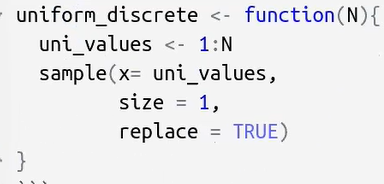
\includegraphics[scale=0.5]{figures/uniform_dis_code}
\end{center}
\section[Binomial Distribution]{Binomial Distribution}
\begin{defn}
We say a random variable X with parameters\begin{align*}
n &\rightarrow \text{ Sample Size}\\
p&\rightarrow \text{ Probability of getting a success}
\end{align*}
has the \textbf{Binomial Distribution} if \begin{align*}
X&=\{0,1,2,\cdots,N\}\\
\forall k\in X,p_X(k)&=\binom nk \cdot p^k \cdot (1-p)^{n-k}
\end{align*}
\end{defn}
\begin{thm}
\textbf{Binomial Theorem}\\
\begin{align*}
(x+y)^n&=\sum_{k=0}^{n}\binom nk x^{n-k}y^k\\
&=\sum_{k=0}^{n}\binom nk x^ky^{n-k}\\
\end{align*}
\end{thm}
\note The experiment is performing n-independent with exactly two outcomes: success, failure. And  p(success)$\in (0,1)$\\
\hfill\\
First, we want to calculate the $p_X(k)$  
Recall $X=\{0,1,2,3,\cdots, n\}$, $P(X=k)=P$( there are exactly k success in n independent trials.\\
$|\{X=k\}=$ number of ways to select n objects from the set $\{S,F\}$. Think of in n boxes, we choose k boxes that will contain the S. This is $\binom nk$ ways.\\
The number of all subsets of a set containing n elements is $2^n$\\
\note $\bigcup_{i=0}^{k}|\{X=k\}|=2^n$\\
\hfill\\
Note that each way has $(p)^{k}(1-p)^{n-k}$ probability, so the total probability and the probability mass function is \begin{align*}
p_X(k)=P(X=k)=\binom nk \cdot p^k\cdot (1-p)^{n-k}
\end{align*} 
Then, we can check if $P_X$ is a probability mass function. Since $\binom nk \cdot p^k\cdot (1-p)^{n-k}\geq 0$ all the time, so we need check $\sum_{x\in X}p_X(x)=1$\begin{align*}
\sum_{x\in X}p_X(x)&=\sum_{k=0}^{n}\binom nk \cdot p^k\cdot (1-p)^{n-k}\\
&=(p+(1-p))^n&\text{By Binomial Theorem}\\
&=1^n\\
&=1
\end{align*} 
Now, we can calculate the \textbf{Expected Value} of X$\sim$Binom(n, p)
\begin{align*}
E(X)&=\sum_{x\in X}x\cdot p_X(x)=\sum_{k=0}^{n}k\cdot p_x(k)\\
&=\sum_{k=0}^{n}k\cdot \binom nk p^k\cdot (1-p)^{n-k}\\
&=\sum_{k=1}^{n}k\cdot \frac{n!}{(n-k)!k!} p^k\cdot (1-p)^{n-k}\\
&=\sum_{k=1}^{n}\frac{n!}{(n-k)!(k-1)!} p^k\cdot (1-p)^{n-k}\\
&=\sum_{k=1}^{n}n\cdot p \frac{(n-1)!}{(n-k)!(k-1)!} p^{k-1}\cdot (1-p)^{n-k}\\
&=n\cdot p \cdot \sum_{k=1}^{n}\frac{(n-1)!}{(n-k)!(k-1)!} p^{k-1}\cdot (1-p)^{n-k}\\
&=n\cdot p \cdot \sum_{r=0}^{n-1}\frac{(n-1)!}{(n-r-1)!(r)!} \cdot p^{r}\cdot (1-p)^{n-r-1} &\text{set }r=(k-1)\\
&=n\cdot p \cdot \sum_{r=0}^{n-1}\frac{(n-1)!}{((n-1)-r)!(r)!} \cdot p^{r}\cdot (1-p)^{(n-1)-r} \\
&=n\cdot p \cdot \sum_{r=0}^{n-1}\binom{n-1}{r}  \cdot p^{r}\cdot (1-p)^{(n-1)-r} \\
&=n p 
\end{align*}
\note $\sum_{r=0}^{n-1}\binom{n-1}{r}  \cdot p^{r}\cdot (1-p)^{(n-1)-r}$ is a probability mass function of Binom$(n-1,p)$, which is the sum of all probability from Binom$(n-1,p)$. By the definition of a probability mass function, it is 1.\\
\hfill\\
Then, let's calculate the \textbf{Variance}
 \begin{align*}
E(X^2)&=\sum_{k=0}^n k^2\cdot p_X(k)=\sum_{k=0}^{n}k^2\cdot \binom nk p^k\cdot (1-p)^{n-k}\\
&=\sum_{k=1}^{n}k^2 \cdot \frac{n!}{(n-k)!k!} p^k\cdot (1-p)^{n-k}\\
&=\sum_{k=1}^{n}k\cdot \frac{n!}{(n-k)!(k-1)!} p^k\cdot (1-p)^{n-k}\\
&=\sum_{k=1}^{n}k\cdot n \cdot p \frac{(n-1)!}{(n-k)!(k-1)!} p^{k-1}\cdot (1-p)^{n-k}\\
&= n \cdot p\sum_{k=1}^{n}k\cdot \binom{n-1}{k-1}\cdot p^{k-1}\cdot (1-p)^{n-k}\\
&= n \cdot p\sum_{k=1}^{n}(r+1)\cdot \binom{n-1}{r}\cdot p^{r}\cdot (1-p)^{(n-1)-r}&\text{Set } r=k-1\\
&=n\cdot p \left( \sum_{r=0}^{n-1}r\binom{n-1}{r}p^r\cdot (1-p)^{(n-1)-r}+\sum_{r=0}^{n-1}\binom{n-1}{r}p^r\cdot (1-p)^{(n-1)-r} \right)\\
&=n\cdot p((n-1)p+1)\\
&=n(n-1)p^2+np
\end{align*}
Then the \textbf{variance} is
\begin{align*}
V(X)&=E(X^2)-E(X)^2\\
&=n(n-1)p^2+np-(np)^2\\
&=np((n-1)p+1-np)\\
&=np(np-p+1-np)\\
&=np\cdot (1-p)
\end{align*}
Then, we can calculate the \textbf{Moment Generating Function} \begin{align*}
M_X(t)&=E(e^{tx})\\
&=\sum_{k=0}^n e^{tk}\cdot p_X(k)\\
&=\sum_{k=0}^{n}e^{tk}\cdot \binom nk p^k\cdot (1-p)^{n-k}\\
&=\sum_{k=0}^{n}e^{tk} \cdot \binom nk \cdot p^k\cdot (1-p)^{n-k}\\
&=\sum_{k=0}^{n}\binom nk  \cdot (e^tp)^k\cdot (1-p)^{n-k}\\
&=(pe^t+(1-p))^n &\text{By Binomial Theorem}
\end{align*}
Using the moment generating function, we can find the $E(X)$. But first we need to find
\begin{align*}
\frac{d}{dt}\left(M_X(t) \right)&=\frac{d}{dt}((pe^t+(1-p))^n)\\
&=n\cdot ((pe^t+(1-p))^{n-1}\cdot pe^t &\text{Chain Rule}
\end{align*}
Then
 \begin{align*}
E(X)&=\frac{d}{dt}\left. \left(M_X(t) \right)\right|_{t=0}\\
&=\left. n\cdot ((pe^t+(1-p))^{n-1}\cdot pe^t \right|_{t=0}\\
&=n\cdot ((p+(1-p))^{n-1}\cdot p\\
&=np
\end{align*}
\color{Red}\textbf{Special Case:} \textbf{Bernoulli Distribution}\\
\color{black}When $n=1$, $X=\{0,1\}, p\in(0,1)$, then \begin{center}
$p_X(x)=\begin{cases}p &x=1\\ (1-p)&x=0 
\end{cases}$
\end{center}
\section[Hyper Geometric Distribution]{Hyper Geometric Distribution}
\begin{defn}
We say a random variable X with parameters \begin{align*}
N&=\text{ population size}\\
M&=\text{ number successes in the population}\\
n&=\text{ sample size}
\end{align*}
is a \textbf{hypergeometric distribution} if and only if \begin{align*}
X&=\{0,1,2,\cdots,min(n,M)\}\\
p_X(k)&=\frac{\binom Mk \cdot \binom{N-M}{n-k}}{\binom{N}{n}}
\end{align*}
\end{defn}
In this setting, $X$ is the number of successes in a sample of size n, sampled from a population of size N with M success and sampling without replacement.\\
$|\{X=k\}|=$ number elements in this set, the number of ways to sample out a sample with exactly k success.\\
 This is same as first find the exactly k success in M successes. And select $(n-k)$ spots with Failure, then fill the rest to failure.\begin{align*}
 \binom Mk \binom{N-M}{n-k}
 \end{align*}
\hfill\\
And the total number of ways to n objects from N without replacements is $\binom Nn$, so we got \begin{align*}
p_X(k)=P(X=k)&=\frac{|\{X=k\}|}{|S|}\\
&=\frac{\binom Mk \cdot \binom{N-M}{n-k}}{\binom{N}{n}}
\end{align*}
The \textbf{Expected Value} is\begin{align*}
E(X)&=n\cdot \left( \frac{M}{N}\right)
\end{align*}
The \textbf{Variance }is \begin{align*}
V(X)&=\frac{N-n}{N-1}\cdot n \cdot \frac{M}{N}\cdot \left( 1-\frac{M}{N}\right)
\end{align*}

\hfill\\
\hfill\\
\hfill\\
\hfill\\
\example 
\textbf{Experiment:} Suppose a bag has N balls. M balls are Blue, $(N-M)$ balls are Red. We draw n balls from this bag.\\
If we are sampling with replacement, then it is a \textbf{binomial distribution} with parameters \begin{align*}
n &\rightarrow \text{ Sample Size}\\
p=\frac{M}{N}&\rightarrow \text{ Probability of getting a success}
\end{align*}
\hfill\\
If we are sampling without replacement, then it is a \textbf{Hypergeometric Distribution} with parameters \begin{align*}
N &\rightarrow \text{ Population}\\
M &\rightarrow \text{ Number success in the population}\\
n &\rightarrow \text{ Sample Size}
\end{align*}
\section{Geometric Distribution}
\begin{defn}
We say X is a geometric distribution if \begin{align*}
X&=\{1,2,3,4,\cdots\}\\
p_X(x)&=p(1-p)^{x-1},x\in X
\end{align*}
Where X = number of trials until a success.
\end{defn}
We can find the moment generating function of X \\
\begin{align*}
M_X(t)&=E(e^{tX})\\
&=\sum_{x\in X} e^{tx}\cdot p_X(x)\\
&=\sum_{k=1}^{\infty}e^{tk}\cdot (1-p)^{k-1}\cdot p\\
&=p\cdot \sum_{k=1}^{\infty}e^{t(k-1)+t}\cdot (1-p)^{k-1}\\
&=p\cdot \sum_{k=1}^{\infty}e^{t}\cdot e^{t(k-1)}\cdot (1-p)^{k-1}& a^x\times a^y=a^{x+y}\\
&=p\cdot  e^{t}\cdot \sum_{k=1}^{\infty} e^{t(k-1)}\cdot (1-p)^{k-1}\\
&=p\cdot  e^{t}\cdot \sum_{k=1}^{\infty} (e^t(1-p))^{k-1} & (ab)^x=a^xb^x\\
&=p\cdot  e^{t}\cdot \sum_{n=0}^{\infty} (e^t(1-p))^{n} & n=k-1\\
&= p\cdot  e^{t}\cdot \left( \frac{1}{1-e^t(1-p)}\right) & \sum_{n=0}^{\infty} a^n =\frac{1}{1-a} \text{ if }|a|<1, \text{ else diverge}\\
&= \frac{ p\cdot  e^{t}}{1-e^t(1-p)} 
\end{align*} 
Therefore,
\begin{align*}
M_X(t)=\frac{ p\cdot  e^{t}}{1-e^t(1-p)} 
\end{align*}
By theorem \textbf{2.4} in chapter 3, we can find the expected value of X using the moment generating function of X. \begin{align*}
\frac{d}{dt}M_X(t)&=\frac{d}{dt}\left( \frac{ p\cdot  e^{t}}{1-e^t(1-p)}  \right)\\
&=\frac{ pe^{t}\cdot (1-e^t(1-p))-pe^t\cdot (-e^t(1-p))}{(1-e^t(1-p))^2} & \text{quotient rule and difference rule}
\end{align*}
We need to evaluating at $t=0$ \begin{align*}
M_X&=E(X)\\
&=\left. \left(\frac{d}{dt}M_X(t)\right) \right|_{t=0}\\
&=\frac{ p (1-(1-p))-pe^t\cdot (-(1-p))}{(1-(1-p))^2}\\
&=\frac{p^2+p-p^2}{p^2}\\
&=\frac{p}{p^2}=\frac{1}{p}
\end{align*}
We can also calculate the $E(X)$ without using moment generation function. Refers back to \textbf{theorem 2.1} in chapter 3, we will get the same result as above\\
\begin{align*}
E(X)&=\sum_{x\in X}x\cdot p_X(x)\\
&=\sum_{k=1}^{\infty}k\cdot p_X(x)\\
&=\sum_{k=1}^{\infty}k\cdot (1-p)^kp\\
&=p\cdot \sum_{k=1}^{\infty}k(1-p)^{k-1}\\
&=p\cdot  \sum_{k=0}^{\infty}k(q)^{k-1}&\text{set }q=1-p\\
&=p\cdot  \frac{d}{dq} \sum_{k=0}^{\infty}(q)^{k}& \frac{d}{dx}(x^n)=nx^{n-1}\\
&=p\cdot \frac{d}{dq} \left( \frac{1}{1-q}\right)=p\cdot \frac{d}{dq} \left( (1-q)^{-1}\right)\\
&=p\cdot -(1-q)^{-2}\cdot -1 &\text{Chain Rule } \frac{d}{dx}[f(g(x))]=f'(g(x))g'(x)\\
&=p\cdot \frac{1}{(1-(1-p))^2}\\
&=\frac{p}{p^2}=\frac{1}{p}
\end{align*}
Using \textbf{Theorem 2.5} in chapter 3, we can calculate the the Variance $V(x)$, first we need to calculate $E(x^2)$\begin{align*}
\frac{d}{dt}\frac{d}{dt}M_X(t)&=\frac{d}{dt}\frac{ pe^{t}\cdot (1-e^t(1-p))-pe^t\cdot (-e^t(1-p))}{(1-e^t(1-p))^2} \\
&=\frac{d}{dt}\frac{ pe^{t}-pe^t\cdot e^t(1-p))-pe^t\cdot -e^t (1-p))}{(1-e^t(1-p))^2} \\
&=\frac{d}{dt}\frac{ pe^{t}-pe^t\cdot e^t(1-p))+pe^t\cdot e^t (1-p))}{(1-e^t(1-p))^2} \\
&=\frac{d}{dt}\frac{ pe^{t}}{(1-e^t(1-p))^2} \\
&=\frac{pe^t(1-e^t(1-p))^2-pe^t\cdot 2(1-e^t(1-p))\cdot (-e^t(1-p))}{(1-e^t(1-p))^4}
\end{align*}
Then, we evaluating at $t=0$\begin{align*}
E(X^2)&=\left. \left(\frac{d}{dt} \frac{d}{dt}M_X(t)\right) \right|_{t=0}\\
&=\frac{p(1-(1-p))^2-p\cdot 2(1-(1-p))\cdot (-(1-p))}{(1-(1-p))^4}\\
&=\frac{p\cdot p^2-p\cdot 2p\cdot (-1+p))}{(p^4}\\
&=\frac{p^2(p-2\cdot (-1+p))}{p^4}\\
&=\frac{(p-2\cdot (-1+p))}{p^2}\\
&=\frac{(p+2\cdot (1-p))}{p^2}\\
\end{align*}
Refers back to \textbf{Theorem 2.5} in chapter 3\begin{align*}
V(X)&=E(X^2)-(E(x))^2\\
&=\frac{(p+2\cdot (1-p))}{p^2}-\frac{1}{p^2}\\
&=\frac{p+2-2p-1}{p^2}\\
&=\frac{p+1-2p}{p^2}=\frac{1-p}{p^2}
\end{align*}
\section[The Negative Binomial Distribution]{The Negative Binomial Distribution}
From now, the examples can take infinitely many values. In particular, the distributions with infinite values are calculating possibilities of events where one is waiting for something to happen.\begin{defn}
We say X with parameters\begin{align*}
p&=\text{Probability of a success}\\
r&=\text{Number of successes we are waiting for}
\end{align*}
 has the \textbf{Negative Binomial Distribution} if\begin{align*}
 X&=\{0,1,2,3,\cdots\}\\
 p_X(k)&=\binom{k+r-1}{r-1}p^r\cdot (1-p)^k\\
 &=\binom{k+r-1}{k}p^r\cdot (1-p)^k\\
 \end{align*}
\end{defn}
\begin{thm}
\textbf{Sum of Negative Binomial Series:}\begin{align*}
(1-w)^{-r}&=\sum_{k=0}^{\infty}\binom{k+r-1}{r-1}w^k
\end{align*}
\end{thm}
To understand Negative Binomial Distribution and  how we got the probability mass function, we could consider the following experiment.\\
\hfill\\
\textbf{Experiment:} Keep tossing a coin independently, fix $r\in \mathbb{R}$, $p(H)\in (0,1)$\\
\text{\qquad} \qquad \qquad $X=$ number of tails until exactly r heads have appeared\\
\text{\qquad} \qquad \qquad OR: Perform a trial whose outcomes are successes independently, $p(S)\in (0,1)$\\
\text{\qquad} \qquad \qquad $X=$ number of failure until exactly r successes have appeared\\
\hfill\\
We want to calculate the probability mass function of X. Note that the values of $\{X=x\}=\{0,1,2,3,\cdots,x\}$\\
\hfill\\
For example, If $r=2$\\
$\{X=0\}=\{$ All outcomes with 0 failures until 2 successes$\}=\{SSS\}$\\
$\{X=0\}=\{$ All outcomes with 1 failures until 2 successes$\}=\{FSS,SFS\}$\\
\hfill\\
Observe: All outcomes in the set $\{X=k\}$ is equally likely, so we first, We find the probability of a single outcome in $\{X=k\}$\begin{center}
$\{X=k\}=\{$All outcomes with exactly k failures before the $r^{th}$ success$\}$
\end{center}
Then, we consider a single event $\omega$ in the set $\{X=k\}$\begin{align*}
\omega &= FFF\cdots F_kSSS\cdots S_r\\ 
\text{Since }P(S)&=p,\text{ }P(F)=(1-p)\\
P(\omega)&=p^{k}p^{r}
\end{align*}
Then, we want to count the $|\{X=k\}|$. \\
Since we need $k+r$ trials for any outcomes in $\{X=k\}$, we can think of having $k+r$ slots,  whereas the last slot $k+r$ will always be S. Then the remaining $(r-1)$ successes can happen in any of the remaining $(k+r-1)$ slots. \\
Therefore we only need to choose $(r-1)$ slots out of $(k+r-1)$ to put the success, which is a total of\begin{align*}
\binom{k+r-1}{r-1}
\end{align*}
or, if we choose the failure seats, we will get \begin{align*}
\binom{k+r-1}{k}
\end{align*}
Therefore, we find that \begin{align*}
|\{X=k\}|=\binom{k+r-1}{r-1}=\binom{k+r-1}{k}=\frac{(k+r-1)!}{(r-1)!k!}
\end{align*}
So the probability mass function is \begin{align*}
p_X(k)=\binom{k+r-1}{r-1}p^r\cdot (1-p)^k
\end{align*}

\hfill\\
Now, suppose $X\sim $NegBinom$(p,r)$, we want to calculate the \textbf{Expected Value} E(X)\begin{align*}
E(X)&=\sum_{x\in X}p_X(x)\\
&=\sum_{k=0}^{\infty}k\cdot p_X(k)\\
&=\sum_{k=0}^{\infty}k\cdot \binom{k+r-1}{k} \cdot p^r\cdot (1-p)^k\\
&=\sum_{k=0}^{\infty}k\cdot \frac{(k+r-1)!}{(r-1)!k!} \cdot p^r\cdot (1-p)^k\\
&=\sum_{k=1}^{\infty} \frac{(k+r-1)!}{(r-1)!(k-1)!} \cdot p^r\cdot (1-p)^k\\
&=\sum_{j=0}^{\infty} \frac{(j+1+r-1)!}{(r-1)!(j)!} \cdot p^r\cdot (1-p)^{j+1} \text{\qquad \qquad Set} j=k-1\\
&=\sum_{j=0}^{\infty} r\cdot \frac{(j+(r+1)-1)!}{(r)!(j)!} \cdot \frac{p^{r+1}}{p}\cdot (1-p)^{j}\cdot (1-p)\\
&=\frac{r(1-p)}{p}\cdot \sum_{j=0}^{\infty} \frac{(j+(r+1)-1)!}{(r+1)-1)!(j)!} \cdot p^{r+1}\cdot (1-p)^{j}\\
&=\frac{r(1-p)}{p}\cdot \sum_{j=0}^{\infty} \binom{(j+(r+1)-1)}{j}\cdot p^{r+1}\cdot (1-p)^{j}\\
&=\frac{r(1-p)}{p}
\end{align*}
Note that $\sum_{j=0}^{\infty} \binom{(j+(r+1)-1)}{j}\cdot p^{r+1}\cdot (1-p)^{j}$ is the sum of all the possibilities associated to NegBinom$(r+1,p)$\\
\hfill\\
Similarly, we can find the \textbf{Variance} $V(X)$ to get \begin{align*}
V(x)&=\frac{r(1-p)}{p^2}
\end{align*}
We can also find the \textbf{Moment Generating Function} is\begin{align*}
M_x(t)&=E(e^{tx})\\
&=\sum_{k=0}^{\infty}e^{tk}\cdot p_X(k)\\
&=\sum_{k=0}^{\infty}e^{tk}\cdot \binom{k+r-1}{r-1} \cdot p^r\cdot (1-p)^k\\
&=p^r\cdot \sum_{k=0}^{\infty}\binom{k+r-1}{r-1} \cdot	 (e^t(1-p))^k\\
&=p^r\cdot (1-(1-p)e^t)^{-r}&\text{Above is Negative Binomial Series}\\
&=\left( \frac{p\cdot e^t}{1-(1-p)e^t}\right)^r
\end{align*}
Therefore, we got
 \begin{align*}
M_x(t)&=\left( \frac{p\cdot e^t}{1-(1-p)e^t}\right)^r
\end{align*}
\newpage
\section[Poisson Distribution]{Poission Distribution}
\note \begin{align*}
e^{\lambda}&=1+\lambda+\frac{\lambda ^2}{2!}+\frac{\lambda^3}{3!}+\cdots\\
&=\sum_{k=0}^{\infty}\frac{\lambda^k}{k!}\\
\hfill\\
\therefore 1&=e^{-\lambda}\sum_{k=0}^{\infty}\frac{\lambda^k}{k!}=\sum_{k=0}^{\infty}\left( \frac{e^{-\lambda}\lambda^k}{k!}\right)
\end{align*}
So we can use to define a probability mass function since it satisfies the requirement of probability mass function.
\begin{defn}
We say X with parameters \begin{align*}
\lambda &\rightarrow \text{rate}
\end{align*}
has the \textbf{Poission Distrubution} if \begin{align*}
X&=\{0,1,2,3,\cdots\}\\
p_X(k)&=e^{-\lambda}\frac{\lambda^k}{k!}
\end{align*}
\end{defn}
We can calculate the \textbf{Expected Value}
\begin{align*}
E(x)&=\sum_{k=0}^{\infty}k\cdot p_X(k)\\
&=\sum_{k=0}^{\infty}k\cdot e^{-\lambda}\cdot \frac{\lambda^k}{k!}\\
&=\sum_{k=1}^{\infty} e^{-\lambda}\cdot \frac{\lambda^k}{(k-1)!}\\
&= \sum_{k=1}^{\infty} e^{-\lambda}\cdot \frac{\lambda^k}{(k-1)!}\\
& =\sum_{j=0}^{\infty} e^{-\lambda}\cdot \frac{\lambda^{j+1}}{(j)!}&\text{Set} j =k-1\\
&=\sum_{j=0}^{\infty} e^{-\lambda}\cdot \lambda\cdot \frac{\lambda^{j}}{(j)!}\\
&=\lambda\cdot \sum_{j=0}^{\infty} e^{-\lambda}\cdot \frac{\lambda^{j}}{(j)!}\\
&=\lambda
\end{align*}
To calculate the \textbf{Variance} $V(x)$, we first need to find $E(X^2)$\begin{align*}
E(X^2)&=\sum_{k=0}^{\infty}k^2\cdot p_X(k)
=\sum_{k=0}^{\infty} k^2 \cdot e^{-\lambda}\cdot \frac{\lambda^k}{k!}\\
&=\lambda\sum_{k=1}^{\infty}ke^{-\lambda}\cdot \frac{-\lambda^k}{(k-1)!}\\
&=\lambda\sum_{j=0}^{\infty}(j+1)e^{-\lambda}\cdot \frac{-\lambda^k}{(j)!}\text{ \qquad \qquad Set}j=k-1\\
&=\lambda \sum_{j=0}^{\infty} j\cdot e^{-\lambda}\cdot \frac{-\lambda^k}{(j)!}+\lambda \sum_{j=0}^{\infty}e^{-\lambda}\cdot \frac{-\lambda^k}{(j)!}\\
&=\lambda \cdot \lambda +\lambda\\
&=\lambda^2 +\lambda
\end{align*}
Then, we can get
\begin{align*}
V(X)&=E(X^2)-E(X)^2\\
&=\lambda^2+\lambda-\lambda^2=\lambda
\end{align*}
Finally, we can calculate the \textbf{Moment Generating Function} $M_X(t)$\begin{align*}
M_X(t)&=\sum_{k=0}^{\infty}e^{tk}\cdot e^{-\lambda}\cdot\frac{\lambda^k}{k!}\\
&=e^{-\lambda}\sum_{k=0}^{\infty}\frac{(e^t\cdot \lambda)^k}{k!}\\
&=e^{-\lambda}\cdot e^{e^t\cdot \lambda} &\text{Note }\sum_{x=0}^{\infty}\frac{a^x}{x!}=e^a\\
&=e^{\lambda(e^t-1)}
\end{align*}
\chapter[Continuous Random Variable]{Continuous Random Variable}
Recall that \begin{defn}
Suppose X is a random variable with cumulative density function $F_X$, i.e\begin{align*}
F_X(x)=P(X\leq x),\text{\qquad}x\in \mathbb{R}
\end{align*}
We say X is a \textbf{continuous random variable} if and only if $F_x$ is a continuous function.\\
\hfill\\
And if there exists a $f_X:\mathbb{R}\rightarrow \mathbb{R}$ such that \begin{align*}
F_X(x)&=\int_{-\infty}^{x}f_X(t)dt\text{\qquad}\forall x\in \mathbb{R}
\end{align*}
We call $f_X$ a \textbf{probability density function for X}
\end{defn}
\note Given a random variable X, there can be multiple probability density functions associated to X\\
\hfill\\
\begin{defn}
We say two random variables, $X,Y$ with cumulative density function $F_X,F_Y$ respectively are identically distributed if \begin{align*}
F_X(u)&=F_Y(u)\text{\qquad} \forall u\in \mathbb{R}
\end{align*}
\end{defn}
\begin{thm}
Given X a continuous random variable with cumulative density function $F_X(x)$ and suppose a probability density function $f_x(x)$ exists. Then \begin{align*}
E(X)&=\int_{-\infty}^{\infty}x\cdot f_X(x)dx\\
V(X)&=\int_{-\infty}^{\infty}(x-M_X)^2\cdot f_X(x)dx\\
M_X(t)&=\int_{-\infty}^{\infty}e^{tx}\cdot f_X(x)dx
\end{align*}
if the integrals exists.
\end{thm}
\begin{thm}
Suppose X is a random variable, and $a,b\in \mathbb{R}$. Let $Y=aX+b$. Then \begin{enumerate}
\item $E(Y)=aE(X)+b$
\item $V(Y)=a^2V(X)$
\item $M_Y(t)=e^{bt}\cdot M_X(at)$
\end{enumerate}
\end{thm}
\begin{proof}
Assume for simplicity that X is continuous with probability density function $f_X(x)$\\
1. $E(Y)=aE(X)+b$ \begin{align*}
E(Y)&=E(aX+b)=\int_{-\infty}^{\infty}(aX+b)f_X(x)dx\\
&=\int_{-\infty}^{\infty}axf_x(x)dx+\int_{-\infty}^{\infty}bf_x(x)dx\\
&=a\int_{-\infty}^{\infty}xf_x(x)dx+b\int_{-\infty}^{\infty}f_x(x)dx\\
&=aE(x)+b
\end{align*}
2.  $V(Y)=a^2V(X)$ \begin{align*}
V(Y)&=V(ax+b)=E((Y-E(Y))^2)\\
Y-E(Y)&=aX+b-(aE(X)+b)=aX-aE(X)=a(X-E(X))\\
V(Y)&=E((a(X-E(X)))^2)\\
&=E(a^2(X-E(X))^2)\\
&=a^2E((X-E(X))^2)\\
&=a^2V(X)
\end{align*}
3.$M_Y(t)=e^{bt}\cdot M_X(at)$\begin{align*}
M_Y(t)&=E(e^{Yt})\\
&=E(e^{(ax+b)t})\\
&=E(e^{axt}\cdot e^{bt})\\
&=e^{bt}\cdot E(e^{X(at)})\\
&=e^{bt}\cdot M_X(at)
\end{align*}
\end{proof}
\section[Uniform Continuous Distribution]{Uniform Continuous Distribution}
\begin{defn}
\textbf{Uniform Continuous Distribution} has parameters \begin{align*}
A,B&\rightarrow \text{end points of an interval}
\end{align*}
with probability density function\begin{align*}
f_X(x;A,B)&=\begin{cases}\frac{1}{B-A} & x\in [A,B]\\ 0 & \text{otherwise}\end{cases}
\end{align*}
\end{defn}
Here is the graph of $f_X(x)$\begin{center}
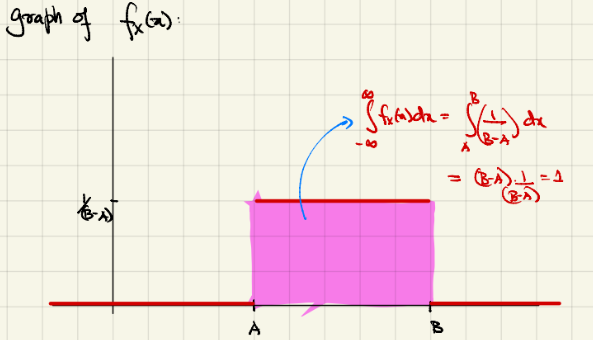
\includegraphics[scale=0.5]{figures/uniform_cont_graph}
\end{center}
Now, we need to see that \begin{align*}
F_X(x)&=\int_{-\infty}^{x}f_X(x)dx
\end{align*}
if $x<A$, then $F_X(x)=0$\\
\hfill\\
if $x\in [A,B]$, then\begin{align*}
F_X(x)&=\int_{-\infty}^{x}f_X(t)dt=\int_{A}^{x}\frac{1}{(B-A)}dt\\
&=\left. \frac{t}{(B-A)}\right|_{A}^{x} =\frac{x-A}{B-A}\\
&=\frac{1}{B-A}x-\frac{A}{(B-A)}\\
\end{align*} 
note that $\frac{1}{B-A}$ is the slope and $-\frac{A}{(B-A)}$ is the y-intercept.\\
\hfill\\
if $x>B$, \begin{align*}
F_X(x)&=\int_{-\infty}^{x}f_X(x)dx\\
&=\int_{A}^{B} \frac{1}{(B-A)}+\int_{B}^{x}0dx\\
&=1
\end{align*}
\hfill\\
The graph of the cumulative density function
\begin{center}
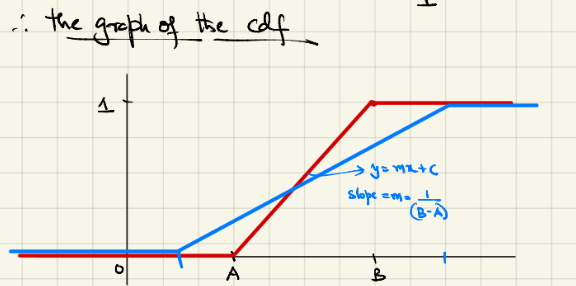
\includegraphics[scale=0.5]{figures/cdf_graph}
\end{center}
\hfill\\
Then, we can calculate the \textbf{Expected Value} $E(X)$\begin{align*}
E(X)&=\int_{-\infty}^{\infty}x\cdot f_X(x)dx=\int_{A}^{B}x\cdot \frac{1}{B-A}dx\\
&=\left. \left( \frac{1}{B-A}\right)\cdot \frac{x^2}{2}\right|_{A}^{B} =\left( \frac{1}{B-A}\right) \left( \frac{B^2-A^2}{2}\right)\\
&=\frac{1}{(B-A)}\frac{(B-A)(B+A)}{2}\\
&=\frac{B+A}{2}
\end{align*}
Then, to calculate the Variance, we first calculate the $E(X^2)$\begin{align*}
E(X^2)&=\int_{-\infty}^{\infty}x^2\cdot f_X(x)dx\\
&=\int_{A}^{B}x^2\cdot \frac{1}{B-A}dx\\
&=\left. \left( \frac{1}{B-A}\right)\cdot \frac{x^3}{3}\right|_{A}^{B}\\
&=\left( \frac{1}{B-A}\right) \left( \frac{B^3-A^3}{3}\right)\\
&=\left( \frac{1}{B-A}\right) \frac{(B-A)(B^2+AB+A^2)}{3}\\
&=\frac{(B^2+AB+A^2)}{3}
\end{align*}
Then, we calculate the \textbf{Variance} $V(X)$\begin{align*}
V(X)&=E(X^2)-(E(X))^2\\
&= \frac{(B^2+AB+A^2)}{3}- \left(\frac{B+A}{2} \right)^2\\
&= \frac{(B^2+AB+A^2)}{3}-\frac{B^2+2AB+A^2}{4}\\
&=\frac{4(B^2+AB+A^2)-3(B^2+2AB+A^2)}{12}\\
&=\frac{4B^2+4AB+4A^2-3B^2-3AB-3A^2}{12}\\
&=\frac{B^2-2AB+A^2}{12}=\frac{(B-A)^2}{12}
\end{align*}
Now, lets calculate the \textbf{Moment Generating Function} $M_X(t)$\begin{align*}
M_X(t)&=E(e^{tx})\\
&=\int_{-\infty}^{\infty}e^{tx}\cdot f_X(x)dx\\
&=\int_{A}^{B}e^{tx}\cdot \frac{1}{(B-A)}dx\\
&=\left. \frac{1}{(B-A)}\cdot \frac{e^{tx}}{t}\right|_{A}^{B}\\
&=\frac{1}{(B-A)}\cdot \frac{e^{Bt}-e^{At}}{t}\\
&=\frac{e^{Bt}-e^{At}}{t(B-A)}
\end{align*}
\section[Normal Distribution]{\color{DarkOrchid}Standard Normal Distribution\color{black}}
\begin{defn}
We say Z has the standard normal distribution if the probability density function of Z is\begin{align*}
f_Z(z)&=\frac{1}{\sqrt{2\pi}}\cdot e^{-\frac{z^2}{2}},z\in (-\infty,\infty)
\end{align*}
\end{defn}
Lets check that $f_Z$ is a probability density function.\begin{proof}
\hfill\\
i) $f_Z(z)\geq 0, \forall z\in \mathbb{R}$\\
\begin{align*}
e^{\frac{-z^2}{2}}&\geq 0\\
\frac{1}{\sqrt{2\pi}}&\geq 0\\
e^{\frac{-z^2}{2}}\cdot \frac{1}{\sqrt{2\pi}} &\geq 0
\end{align*}
ii) $\int_{-\infty}^{\infty}f_Z(z)dz=1$\\
We want to show that $\int_{-\infty}^{\infty}\frac{1}{\sqrt{2\pi}}\cdot e^{\frac{-z^2}{2}}dz=1$. To do so, let's try the following\begin{align*}
\left( \int_{\infty}^{\infty}e^{\frac{-z^2}{2}}dz \right)^2&=\left(  \int_{\infty}^{\infty}e^{\frac{-z^2}{2}}dz \right)\left( \int_{\infty}^{\infty}e^{\frac{-z^2}{2}}dz \right)\\
&=\left(  \int_{\infty}^{\infty}e^{\frac{-z^2}{2}}dz \right)\left( \int_{\infty}^{\infty}e^{\frac{-y^2}{2}}dy \right)\\
&=\int_{\infty}^{\infty}\int_{\infty}^{\infty}e^{\frac{-z^2}{2}}\cdot e^{\frac{-y^2}{2}}dzdy\\
&=\int_{\infty}^{\infty}\int_{\infty}^{\infty}e^{\frac{-(z^2+y^2)}{2}}dzdy\\
&\text{Then, we can change it to polar coordinate}\\
&=\int_{0}^{2\pi}\int_{0}^{\infty}e^{\frac{-r^2}{2}}rdrd \theta& r^2=r^2+y^2 \text{\qquad} dzdy=rdrd\theta \text{\qquad}0\leq \theta\leq 2\pi \\
&=\int_{0}^{2\pi}\int_{0}^{\infty}e^{\frac{-s}{2}}ds d\theta&s=\frac{r^2}{2} \text{\qquad} ds=\frac{2r}{2}dr=rdr\\
&=\int_{0}^{2\pi}\left(\lim_{c\rightarrow\infty}\int_{0}^{c}e^{\frac{-s}{2}}ds \right)d\theta \\
&=\int_{0}^{2\pi}\left(\lim_{c\rightarrow\infty} \left. \frac{e^{-s}}{-1} \right|_{0}^{c} \right)d\theta \\
&=\int_{0}^{2\pi}\left(\lim_{c\rightarrow\infty} \left(1-e^{-c}\right) \right)d\theta \\
&=\int_{0}^{2\pi}1d\theta\\
&=2\pi 
\end{align*}
So, we know that \begin{align*}
\left( \int_{\infty}^{\infty}e^{\frac{-z^2}{2}dz}\right)^2&=2\pi\\
 \int_{\infty}^{\infty}e^{\frac{-z^2}{2}dz}&=\sqrt{2\pi}\\
  \int_{\infty}^{\infty}\frac{1}{\sqrt{2\pi}}e^{\frac{-z^2}{2}dz}&=1\\
\end{align*}
Therefore, it is a probability density function.
\end{proof}
Here is visualizing the $f_Z(z)$
\begin{center}
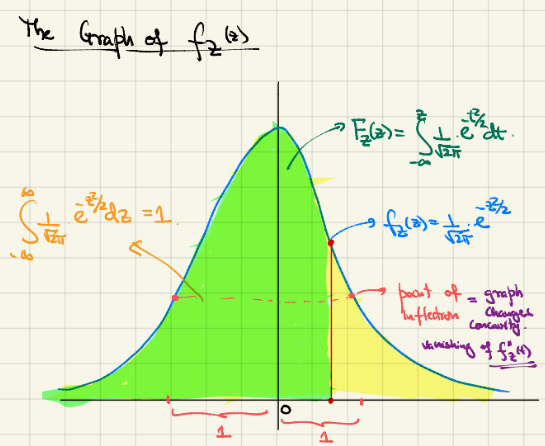
\includegraphics[scale=0.6]{figures/normal_dis_graph}
\end{center}
Also, the cumulative distribution function of the standard normal distribution is \begin{align*}
F_Z(z)&=\int_{-\infty}^{z}f_Z(t)dt=\int_{-\infty}^{z}\int_{\infty}^{\infty}\frac{1}{\sqrt{2\pi}}e^{\frac{-t^2}{2}}dt
\end{align*}
Then, we can calculate the \textbf{Expected Value} $E(Z)$.\begin{align*}
E(Z)&=\int_{-\infty}^{\infty}z\cdot f_Z(z)dz\\
&=\int_{-\infty}^{\infty}z\cdot \frac{1}{\sqrt{2\pi}}e^{\frac{-z^2}{2}}dz\\
&=\int_{-\infty}^{0}z\cdot \frac{1}{\sqrt{2\pi}}e^{\frac{-z^2}{2}}dz+\int_{0}^{\infty}z\cdot \frac{1}{\sqrt{2\pi}}e^{\frac{-z^2}{2}}
\end{align*}
Then, let's first calculate the $\int_{0}^{\infty}z\cdot \frac{1}{\sqrt{2\pi}}e^{\frac{-z^2}{2}}$.\begin{align*}
\int_{0}^{\infty}z\cdot \frac{1}{\sqrt{2\pi}}e^{\frac{-z^2}{2}}&=\lim_{c\rightarrow \infty}\frac{1}{\sqrt{2\pi}}\int_{0}^{C}z\cdot e^{\frac{-z^2}{2}}dz\\
&=\lim_{c\rightarrow \infty}\frac{1}{\sqrt{2\pi}}\int_{0}^{\frac{-c^2}{2}} e^{u}-du &\text{Set }u=\frac{-z^2}{2}\implies du=-zdz\text{\quad}-du=zdz\\
&&z=0\implies u=0\text{\qquad} z=c\implies u=-\frac{c^2}{2}\\
&=\lim_{c\rightarrow \infty}\frac{1}{\sqrt{2\pi}}\left( \left. -e^u\right|_0^{\frac{-c^2}{2}} \right)\\
&=\lim_{c\rightarrow \infty}\frac{-1}{\sqrt{2\pi}}\left(-e^{\frac{-c^2}{2}}+e^0 \right)\\
&=\lim_{c\rightarrow \infty}\frac{1}{\sqrt{2\pi}}\left(1-\frac{1}{e^{\frac{c^2}{2}}} \right)\\
&=\frac{1}{\sqrt{2\pi}}\lim_{c\rightarrow \infty}\left(1-\frac{1}{e^{\frac{c^2}{2}}} \right)=\frac{1}{\sqrt{2\pi}}
\end{align*}
Then, let's calculate the $\int_{-\infty}^{0}z\cdot \frac{1}{\sqrt{2\pi}}e^{\frac{-z^2}{2}}dz$\begin{align*}
\int_{-\infty}^{0}z\cdot \frac{1}{\sqrt{2\pi}}e^{\frac{-z^2}{2}}&=\lim_{c\rightarrow -\infty}\frac{1}{\sqrt{2\pi}}\int_{c}^{0}z\cdot e^{\frac{-z^2}{2}}dz\\
&=\lim_{c\rightarrow -\infty}\frac{1}{\sqrt{2\pi}}\int_{0}^{\frac{-c^2}{2}} e^{u}-du &\text{Set }u=\frac{-z^2}{2}\implies du=-zdz\text{\quad}-du=zdz\\
&&z=0\implies u=0\text{\qquad} z=c\implies u=-\frac{c^2}{2}\\
&=\lim_{c\rightarrow -\infty}\frac{1}{\sqrt{2\pi}}\left( \left. -e^u\right|_{\frac{-c^2}{2}}^{0} \right)\\
&=\lim_{c\rightarrow -\infty}\frac{1}{\sqrt{2\pi}}\left(-e^{\frac{-c^2}{2}}+e^0 \right)\\
&=\lim_{c\rightarrow -\infty}\frac{1}{\sqrt{2\pi}}\left(\frac{1}{e^{\frac{c^2}{2}}}-1 \right)\\
&=\frac{1}{\sqrt{2\pi}}\lim_{c\rightarrow -\infty}\left(0-1 \right)=\frac{1}{-\sqrt{2\pi}}
\end{align*}
Then, \begin{align*}
E(Z)&=\int_{-\infty}^{0}z\cdot \frac{1}{\sqrt{2\pi}}e^{\frac{-z^2}{2}}dz+\int_{0}^{\infty}z\cdot \frac{1}{\sqrt{2\pi}}e^{\frac{-z^2}{2}}\\
&=\frac{1}{\sqrt{2\pi}}+\frac{1}{-\sqrt{2\pi}}=0
\end{align*}
Then, we can calculate the \textbf{Variance}. Since $E(Z)=0$, then $E(Z)^2=0$. \begin{align*}
V(Z)&=E(Z^2)-E(Z)^2\\
&=E(Z^2)\\
&=\int_{-\infty}^{\infty}z^2\cdot f_Z(z)dz\\
&=\int_{-\infty}^{\infty}z^2\cdot \frac{1}{\sqrt{2\pi}}e^{\frac{-z^2}{2}}dz\\
&=\frac{1}{\sqrt{2\pi}}\int_{-\infty}^{\infty}z^2\cdot e^{\frac{-z^2}{2}}dz\\
&=\frac{1}{\sqrt{2\pi}}\left( \int_{-\infty}^{0}z^2\cdot e^{\frac{-z^2}{2}}dz+ \int_{0}^{\infty}z^2\cdot e^{\frac{-z^2}{2}}dz\right)\\
&=\frac{1}{\sqrt{2\pi}}\left(\int_{-\infty}^{0}z^2\cdot e^{\frac{-z^2}{2}}dz+ \int_{0}^{\infty}z^2\cdot e^{\frac{-z^2}{2}}dz\right)\\
&=\frac{1}{\sqrt{2\pi}}\left( \left. uv\right|_{-\infty}^0-\int_{-\infty}^{0}vdu+\left. uv\right|_{0}^{\infty}-\int_{0}^{\infty}vdu \right)\\
&\text{Use Integration By Parts }u=z \text{\quad} dv=z e^{\frac{-z^2}{2}}dz \\
&du=1dz \text{\quad} v=-e^{\frac{-z^2}{2}}\\
&=\frac{1}{\sqrt{2\pi}}\left( \left. z\cdot - e^{\frac{-z^2}{2}}\right|_{-\infty}^{0}  -\int_{-\infty}^{0} -e^{\frac{-z^2}{2}}dz +  \left. z\cdot - e^{\frac{-z^2}{2}}\right|_{0}^{\infty}  -\int_{0}^{\infty} -e^{\frac{-z^2}{2}}dz  \right)\\
&=\frac{1}{\sqrt{2\pi}}\left( \left. z\cdot - e^{\frac{-z^2}{2}}\right|_{-\infty}^{0}  +\int_{-\infty}^{0} e^{\frac{-z^2}{2}}dz +  \left. z\cdot - e^{\frac{-z^2}{2}}\right|_{0}^{\infty}  +\int_{0}^{\infty} e^{\frac{-z^2}{2}}dz  \right)\\
&=\frac{1}{\sqrt{2\pi}}\left((0-0)+(0-0)  +\int_{-\infty}^{\infty} e^{\frac{-z^2}{2}}dz\right)\\
&= \int_{-\infty}^{\infty} \frac{1}{\sqrt{2\pi}} e^{\frac{-z^2}{2}}dz \\
&=e^{\frac{t^2}{2}} \\
&\text{This is the probability density function of standard normal distribution}\\
&=1
\end{align*}
Finally, we can calculate the \textbf{Moment Generating Function} $M_Z(t)$\begin{align*}
M_Z(t)&=E(e^{tz})\\
&=\int_{-\infty}^{\infty}\frac{1}{\sqrt{2\pi}}e^{tz}\cdot e^{-\frac{z^2}{2}}dz\\
&=\int_{-\infty}^{\infty}\frac{1}{\sqrt{2\pi}}\cdot e^{-\left( \frac{z^2}{2}-tz\right)}dz\\
&=\int_{-\infty}^{\infty}\frac{1}{\sqrt{2\pi}}\cdot e^{-\left( \frac{z^2}{2}-tz+\frac{t^2}{2}-\frac{t^2}{2}\right)}dz\\
&=\int_{-\infty}^{\infty}\frac{1}{\sqrt{2\pi}}\cdot e^{-\left( \frac{z^2}{2}-tz+\frac{t^2}{2}\right)}\cdot e^{\frac{t^2}{2}}dz\\
&= e^{\frac{t^2}{2}}\cdot \int_{-\infty}^{\infty}\frac{1}{\sqrt{2\pi}}\cdot e^{-\left( \frac{z^2}{2}-tz+\frac{t^2}{2}\right)}dz\\
&= e^{\frac{t^2}{2}}\cdot \int_{-\infty}^{\infty}\frac{1}{\sqrt{2\pi}}\cdot e^{- \frac{(z-t)^2}{2}}dz\\
&= e^{\frac{t^2}{2}}\cdot \int_{-\infty}^{\infty}\frac{1}{\sqrt{2\pi}}\cdot e^{- \frac{u^2}{2}}dz&\text{Set }u=z-t,\text{\quad}du=dz\\
&\text{Above is a probability density function for standard normal ditsirbution}\\
&= e^{\frac{t^2}{2}}
\end{align*}
\hfill\\
\color{DarkOrchid}{\Large \textbf{Normal Distribution}}\color{black}
\begin{defn}
We say X has the \textbf{Normal Distribution} with parameters \begin{align*}
M&\rightarrow mean\\
\sigma^2&\rightarrow variance
\end{align*}
if the probability density function of X is \begin{align*}
f_X(x)&=\frac{1}{\sqrt{2\pi}\sigma}\cdot e^{\frac{-(x-M)^2}{2\sigma^2}},\text{\qquad}x\in (-\infty,\infty)
\end{align*}
\end{defn}
\hfill\\
Now, let's verify that $f_X(x)$ is a probability density function.\\
i) $f_X(x)\geq 0 \text{\qquad} \forall x$\\
This is the same as the Standard Normal Distribution. So it is verified.\\
\hfill\\
ii) $\int_{-\infty}^{\infty}f_X(x)dx=1$\\
\begin{align*}
\int_{-\infty}^{\infty}f_X(x)dx&=\int_{-\infty}^{\infty}\frac{1}{\sqrt{2\pi}\sigma}\cdot e^{\frac{-(x-M)^2}{2\sigma^2}}\\
&=\int_{-\infty}^{\infty}\frac{1}{\sqrt{2\pi}\sigma}\cdot e^{\left(\frac{-(x-M)}{\sigma}\right)^2\frac{1}{2}}\\
&=\int_{-\infty}^{\infty}\frac{1}{\sqrt{2\pi}}\cdot e^{\frac{-z^2}{2}}dz&Z=\frac{x-M}{\sigma}\implies dz=\frac{dx}{\sigma}\\
&=1&\text{Note it is the pdf of standard normal distribution}
\end{align*}
\begin{defn}
Suppose $X\sim N(M,\sigma^2)$, then \begin{align*}
Z=\frac{X-M}{\sigma}&\longrightarrow \text{Z-Score of X}
\end{align*}
\end{defn}
\note The standard normal distribution has parameters $M=0$ and $\sigma^2=1$, i.e $Z\sim (0,1)$\\
\begin{thm}
Suppose $X\sim N(M,\sigma^2)$ and $Z\sim N(0,1)$. Then \begin{enumerate}
\item $\left( \frac{X-M}{\sigma}\right)\sim N(0,1)$
\item $X=\sigma Z +M$
\end{enumerate}
\end{thm}

\begin{proof}
\begin{align*}
F_{\frac{X-M}{\sigma}}(u)&=P\left( \frac{X-M}{\sigma}\leq u\right)\\
&=P\left( X\leq \sigma u +M\right)\\
&=\int_{-\infty}^{\sigma u +u}\frac{1}{\sqrt{2\pi}\sigma}\cdot e^{\frac{-(x-M)^2}{2\sigma^2}}dx\\
&=\int_{-\infty}^{u}\frac{1}{\sqrt{2\pi}}\cdot e^{\frac{-z^2}{dz}}&Z=\frac{X-M}{\sigma}\text{\qquad}dz=\frac{dx}{\sigma}\\
&=F_Z(u)
\end{align*}
Therefore, $\left(\frac{X-M}{\sigma}\right)$ are identically distributed, meaning $\left(\frac{X-M}{\sigma}\right)$  has the standard normal distribution.
\end{proof}
\begin{thm}
Suppose $X\sim N(M,\sigma^2)$. Note that $X=\sigma Z+M$. Then using the Theorem \textbf{0.2}\begin{align*}
E(X)&=\sigma E(Z)+M=M\\
V(X)&=\sigma^2\cdot V(Z)=\sigma^2\\
M_X(t)&=e^{Mt}\cdot M_Z(\sigma t)\\
&=e^{Mt}\cdot \left( \left. e^{\frac{t^2}{2}}\right|_{t=\sigma t}\right)\\
&=e^{Mt}\cdot e^{\frac{\sigma^2t^2}{2}}\\
&=e^{Mt+\frac{\sigma^2t^2}{2}}
\end{align*}
\end{thm}
\section[Gamma Distribution]{\color{DarkOrchid} Standard Gamma Distribution\color{black}}
\begin{defn}
The \textbf{Gamma Function} is defined as  for $\alpha >0$,\begin{align*}
\Gamma(\alpha)&=\int_{0}^{\infty}t^{\alpha -1}\cdot e^{-t}dt
\end{align*}
\end{defn}
\begin{thm}
Some \textbf{Properties of the Gamma Function}
\begin{enumerate}
\item $\Gamma (\alpha)\geq 0$
\item $\Gamma (\alpha +1)=\alpha \Gamma(\alpha)$
\item $\forall n \in \N,$ $\Gamma(n+1)=n!$ 
\item $\Gamma\left(\frac{1}{2} \right)=\sqrt{\pi}$
\end{enumerate}
\end{thm}
\begin{proof}
1) $\Gamma (\alpha)\geq 0$ \begin{align*}
t^{\alpha -1}&\geq 0,\text{ } t\in(0,\infty)\\
e^{-t}&\geq 0,\text{ } t\in(0,\infty)\\
t^{\alpha -1}\cdot e^{-t}&\geq 0,\text{ } \forall t\in (0,\infty)\\
\text{Then }\int_{0}^{\infty} t^{\alpha -1}\cdot e^{-t}&\geq 0,\text{ }\forall \alpha>0
\end{align*}
2) $\Gamma (\alpha +1)=\alpha \Gamma(\alpha)$\begin{align*}
\Gamma (\alpha +1)&=\int_{0}^{\infty}t^{\alpha+1 -1}\cdot e^{-t}dt\\
&=\int_{0}^{\infty}t^{\alpha}\cdot e^{-t}dt\\
&=uv - \int_{0}^{\infty} udv &\text{Set } v=t^{\alpha}, \text{ }dv=\alpha t^{\alpha -1}dt\\
&&\text{Set } du=e^{-t}, \text{ }u=-e^{-t}\\
&=\left. -t^{\alpha} e^{-t}\right|_{0}^{\infty}-\int_{0}^{\infty}-\alpha t^{\alpha -1}\cdot e^{-t}\\
&=\alpha \int_{0}^{\infty} t^{\alpha -1}\cdot e^{-t}\\
&=\alpha \Gamma(\alpha)
\end{align*}
3) $\forall n \in \N,$ $\Gamma(n+1)=n!$ 
\begin{align*}
\Gamma(1)&=\int_{0}^{\infty}t^{1-1}\cdot e^{-t}dt\\
&=\int_{0}^{\infty}e^{-t}dt\\
&=\lim_{c\rightarrow \infty}\int_{0}^{c}e^{-t}dt\\
&=\lim_{c\rightarrow \infty}\left( \left. \frac{e^{-t}}{-1}\right|_{0}^{c} \right)\\
&=\lim_{c\rightarrow \infty}\left( 1-e^{-c} \right)\\
&=1
\end{align*}
\begin{align*}
\Gamma(n+1)&=n\Gamma(n)\\
&=n\left((n-1)\Gamma(n-1)\right)\\
&\text{\qquad} \vdots\\
&=n(n-1)(n-2)\cdot 3\times 2 \times 1 \times \Gamma(1)\\
&=n!
\end{align*}
4)  $\Gamma\left(\frac{1}{2} \right)=\sqrt{\pi}$\begin{align*}
\Gamma(\frac{1}{2})&=\int_{0}^{\infty}t^{\frac{1}{2}-1}e^{-t}dt\\
&=\int_{0}^{\infty}t^{-\frac{1}{2}}e^{-t}dt\\
&=\int_{0}^{\infty}u^{-1}e^{-u^2}2udu&\text{Set }u=t^{\frac{1}{2}},\text{ }du=\frac{1}{2}t^{-\frac{1}{2}}dt\\
&&dt=2uu^{-1}du,\text{ }e^{-t}=e^{-u^2}\\
&=2\int_{0}^{\infty}e^{-u^2}du\\
&=\int_{-\infty}^{\infty}e^{-u^2}du&e^{-u^2}\text{ is an even function}\\
&=\sqrt{\pi} &\text{Gaussian Integral}
\end{align*}
\end{proof}
\begin{defn}
We say T has the \textbf{Standard Gamma Distribution} with parameter\begin{align*}
\alpha \rightarrow \text{ shape}
\end{align*}
if the probability density function of T is given by \begin{align*}
f_T(t)&=\begin{cases}
\frac{1}{\Gamma(\alpha)}\cdot t^{\alpha -1}\cdot e^{-t}&t>0\\
0&t\leq 0
\end{cases}
\end{align*}
\end{defn}
We need to verify that $f_T$ is in fact a probability density function.\begin{proof}
i) $f_T(t)\geq 0$\begin{align*}
\frac{1}{\Gamma(\alpha)} &\geq 0\\
t^{\alpha-1}&\geq 0 \text{ if } t\in(0,\infty)\\
e^{-t}&\geq 0\\
\text{Then, \qquad }
f_T(t)=\frac{1}{\Gamma(\alpha)}&\cdot t^{\alpha -1}\cdot e^{-t}>0
\end{align*}
ii) $\int_{-\infty}^{\infty}f_T(t)dt=1$\begin{align*}
\int_{-\infty}^{\infty}f_T(t)dt&=\int_{0}^{\infty}\frac{1}{\Gamma(\alpha)}\cdot t^{\alpha -1}\cdot e^{-t}dt\\
&=\frac{1}{\Gamma(\alpha)}\cdot \int_{0}^{\infty}t^{\alpha -1}\cdot e^{-t}dt\\
&=\frac{1}{\Gamma(\alpha)}\cdot \Gamma(\alpha)&\text{By the definition of Gamma function}\\
&=1
\end{align*}
\end{proof}
First, let's calculate \textbf{Expect Value} $E(T)$\begin{align*}
E(T)&=\int_{-\infty}^{\infty}tf_T(t)dt\\
&=\int_{0}^{\infty}t\cdot \frac{1}{\Gamma(\alpha)}\cdot t^{\alpha -1}\cdot e^{-t}dt\\
&=\int_{0}^{\infty} \frac{1}{\Gamma(\alpha)}\cdot t^{\alpha}\cdot e^{-t}dt\\
&= \frac{1}{\Gamma(\alpha)}\cdot \int_{0}^{\infty} t^{\alpha}\cdot e^{-t}dt\\
&= \frac{1}{\Gamma(\alpha)}\cdot \int_{0}^{\infty} t^{\alpha+1-1}\cdot e^{-t}dt\\
&=\frac{1}{\Gamma(\alpha)}\cdot \Gamma(\alpha+1)&\text{Definition of }\Gamma(\alpha+1)\\
&=\frac{1}{\Gamma(\alpha)}\cdot \alpha\Gamma(\alpha)\\
&=\alpha
\end{align*}
Then, let's calculate the \textbf{Variance}. To do so, we need to calculate the $E(T^2)$.\begin{align*}
E(T^2)&=\int_{0}^{\infty}t^2\cdot \frac{1}{\Gamma(\alpha)}\cdot t^{\alpha -1}\cdot e^{-t}dt\\
&=\frac{1}{\Gamma(\alpha)}\cdot \int_{0}^{\infty}t^{\alpha+2-1}\cdot e^{-t}dt\\
&=\frac{1}{\Gamma(\alpha)}\cdot \Gamma(\alpha+2)\\
&=\frac{1}{\Gamma(\alpha)}\cdot (\alpha+1) \Gamma(\alpha+1)\\
&=\frac{1}{\Gamma(\alpha)}\cdot (\alpha+1)(\alpha) \Gamma(\alpha)\\
&=(\alpha+1)(\alpha)
\end{align*}
Then, \begin{align*}
V(T)&=E(T^2)-(E(T))^2\\
&=(\alpha+1)(\alpha)-\alpha^2\\
&=\alpha^2+\alpha-\alpha^2\\
&=\alpha
\end{align*}
Finally, we can calculate the \textbf{Moment Generating Function} $M_T(t)$\begin{align*}
M_T(t)&=E(e^{tT})\\
&=\int_{0}^{\infty}e^{ts}\cdot \frac{1}{\Gamma(\alpha)}\cdot s^{\alpha -1}\cdot e^{-s}ds\\
&= \frac{1}{\Gamma(\alpha)}\cdot \int_{0}^{\infty}e^{ts}\cdot s^{\alpha -1}\cdot e^{-s}ds\\
&= \frac{1}{\Gamma(\alpha)}\cdot \int_{0}^{\infty}e^{-s(1-t)}\cdot s^{\alpha -1}ds\\
&= \frac{1}{\Gamma(\alpha)}\cdot \int_{0}^{\infty}\left( \frac{u}{1-t}\right)^{\alpha-1}\cdot e^{-u}\cdot \frac{du}{1-t}&\text{Set }u=s(1-t)\text{ }du=(1-t)ds\\
&&ds=\frac{du}{(1-t)}\text{ }s=\frac{u}{1-t}\text{ }-s(1-t)=-u\\
&= \frac{1}{\Gamma(\alpha)}\cdot \int_{0}^{\infty}\frac{u^{\alpha-1}}{(1-t)^{\alpha-1}}\cdot e^{-u}\cdot \frac{du}{1-t}\\
&= \frac{1}{(1-t)^{\alpha}}\cdot \frac{1}{\Gamma(\alpha)}\cdot \int_{0}^{\infty}u^{\alpha-1}\cdot e^{-u}\cdot du\\
&= \frac{1}{(1-t)^{\alpha}}\cdot \frac{1}{\Gamma(\alpha)}\cdot \Gamma(\alpha)&\text{Above is }\Gamma(\alpha)\\
&=\frac{1}{(1-t)^{\alpha}}
\end{align*}
Suppose $T\sim Gamma(\alpha),$ $\alpha>0$. This is a Gamma distribution with shape$=\alpha$. Then for $\beta>0$, we define \begin{align*}
X=\beta T
\end{align*}
X is T scaled by a factor of $\beta$. We want to calculate the probability density function of X using the probability density function of T.\\
\hfill\\
First, we calculate the cumulative density function of X, i.e $F_x$\begin{align*}
F_X(x)&=P(X\leq x)\\
&=P(\beta T\leq x)\\
&=P(T\leq \frac{x}{\beta})\\
&=\int_{0}^{\frac{x}{\beta}}f_{T}(t)dt\\
&=F_T\left(\frac{x}{\beta} \right)\\
&=\int_{0}^{\frac{x}{\beta}}\frac{1}{\Gamma(\alpha)}\cdot t^{\alpha -1}\cdot e^{-t}dt
\end{align*}
Then, we differentiate $F_X$ to get $f_X$.\begin{align*}
f_X(x)&=\frac{d}{dx}(F_X(x))\\
&=\frac{d}{dx}\left( \int_{0}^{\frac{x}{\beta}}\frac{1}{\Gamma(\alpha)}\cdot t^{\alpha -1}\cdot e^{-t}dt\right)\\
&=\frac{d}{dx}\left( \frac{x}{\beta}\right)\cdot g(b(x))-\frac{d}{dx}(0)\cdot g(0)\\
&=\frac{1}{\beta}\cdot \frac{1}{\Gamma(\alpha)}\cdot \left( \frac{x}{\beta}\right)^{\alpha-1}\cdot e^{-\left( \frac{x}{\beta}\right)}\\
&=\frac{1}{\Gamma(\alpha)\beta}\cdot \left( \frac{x}{\beta}\right)^{\alpha-1}\cdot e^{-\left( \frac{x}{\beta}\right)}\\
\end{align*} 
\color{DarkOrchid}{\Large \textbf{Gamma Distribution}}\color{black}
\begin{defn}
We say X has the \textbf{Gamma Distribution} with parameters\begin{align*}
\alpha>0 &\rightarrow \text{Shape}\\
\beta>0 &\rightarrow \text{Scale}
\end{align*}
if X has the probability density function defined as \begin{align*}
f_X(x)&=\begin{cases}
\frac{1}{\Gamma(\alpha)\cdot \beta^{\alpha}}\cdot x^{\alpha-1}\cdot e^{\frac{-x}{\beta}}&x>0\\
0&x\leq 0
\end{cases}
\end{align*}
\end{defn}
Now, Let's Check that $f_X(x)$ is a probability density function. \begin{proof}
i) $f(x)\geq 0$\\
This is same as the Standard Gamma Distribution.\\
\hfill\\
ii) $\int_{-\infty}^{\infty}f_X(x)dx=1$\begin{align*}
\int_{-\infty}^{\infty}f_X(x)dx&=\int_{0}^{\infty} \frac{1}{\Gamma(\alpha)\cdot \beta^{\alpha}}\cdot x^{\alpha-1}\cdot e^{\frac{-x}{\beta}}dx\\
&=\frac{1}{\Gamma(\alpha)\cdot \beta^{\alpha}}\int_{0}^{\infty}  (\beta u)^{\alpha-1}\cdot e^{-u}\beta du &\text{Set }u=\frac{x}{\beta}\text{\quad }du=\frac{dx}{\beta}\\
&&x=\beta u\text{\quad} dx=\beta du\\
&=\frac{1}{\Gamma(\alpha)\cdot \beta^{\alpha}}\int_{0}^{\infty}  (\beta)^{\alpha}(u)^{\alpha-1}\cdot e^{-u}du\\
&=\frac{1}{\Gamma(\alpha)}\int_{0}^{\infty} (u)^{\alpha-1}\cdot e^{-u}du&\text{This is }\Gamma(\alpha)  \\
&=\frac{1}{\Gamma(\alpha)}\Gamma(\alpha)=1
\end{align*}
\end{proof}
First, we calculate the \textbf{Expected Value} $E(X)$. Note that $X=\beta T$, then \begin{align*}
E(X)&=E(\beta T)\\
&=\beta \cdot E(T)=\beta \cdot \alpha
\end{align*}
Then, we calculate the \textbf{Variance} $V(X)$. \begin{align*}
V(X)&=V(\beta T)\\
&=\beta^2\cdot V(T)\\
&=\beta^2\cdot \alpha
\end{align*}
Lastly, we calculate the \textbf{Moment Generating Function} $M_X(t)$\begin{align*}
M_X(t)&=M_{\beta T}(t)\\
&=M_T(\beta t)\\
&=\left(\frac{1}{1-\beta t} \right)^{\alpha}
\end{align*}
The Gamma distribution $X\sim Gamma(\alpha,\beta)$ has two important \textbf{special cases}.\\
\hfill\\
When $\alpha=1$, it is a \textbf{Exponential Distribution} with $\lambda = \frac{1}{\beta}$.\\
When $\beta =2$, it is a \textbf{Chi-Squared Distribution} with $\nu=2\alpha$\\
\hfill\\
\section[Exponential Distribution]{\color{DarkOrchid}Exponential Distribution\color{black}}
\begin{defn}
We say X has the \textbf{Exponential Distribution} with parameters\begin{align*}
\alpha &\rightarrow \text{Rate Parameter}
\end{align*}
if X has the probability density function defined as \begin{align*}
f_X(t)&=\begin{cases}
\lambda \cdot e^{-\lambda t}&t>0\\
0&t\leq 0
\end{cases}
\end{align*}
\end{defn}
Note that this is same as Gamma Distribution with $\alpha=1,\beta=\frac{1}{\lambda}$\\
Then, the \textbf{Expected Value }$E(X)$\begin{align*}
E(X)&=\alpha \cdot \beta \\
&=1\cdot \frac{1}{\lambda}\\
&=\frac{1}{\lambda}
\end{align*}
The \textbf{Variance} $V(X)$ is \begin{align*}
V(X)&=\alpha \cdot \beta^2=\frac{1}{\lambda^2}
\end{align*}
The \textbf{Moment Generating Function} $M_X(t)$ is \begin{align*}
M_X(t)&=\left(\frac{1}{1-t\beta} \right)^{\alpha}\\
&=\frac{1}{1-t\cdot\frac{1}{\lambda}}\\
&=\frac{\lambda}{\lambda-t}
\end{align*}
\section[Chi-Squared Distribution]{\color{DarkOrchid}Chi-Squared Distribution\color{black}}
\begin{defn}
We say X has the \textbf{Chi-Squared Distribution} with parameters\begin{align*}
\nu &\rightarrow \text{Rate Parameter}
\end{align*}
if X has the probability density function defined as \begin{align*}
f_X(x)&=\begin{cases}
\frac{1}{\Gamma\left(\frac{\nu}{2}\right)\cdot 2^{\frac{\nu}{2}}}\cdot x^{\frac{\nu}{2}-1}\cdot e^{\frac{-x}{2}}&x>0\\
0&x\leq 0
\end{cases}
\end{align*}
\end{defn}
Note that this is same as Gamma Distribution with $\alpha=\frac{\nu}{2},\beta=2$\\
Then, the \textbf{Expected Value }$E(X)$\begin{align*}
E(X)&=\alpha \cdot \beta \\
&=2\cdot \frac{\nu}{2}\\
&=\nu
\end{align*}
The \textbf{Variance} $V(X)$ is \begin{align*}
V(X)&=\alpha \cdot \beta^2\\
&=2^2\cdot \frac{\nu}{2}\\
&=2\nu
\end{align*}
The \textbf{Moment Generating Function} $M_X(t)$ is \begin{align*}
M_X(t)&=\left(\frac{1}{1-t\beta} \right)^{\alpha}\\
&=\left(\frac{1}{1-2t}\right)^{\frac{\nu}{2}}\\
\end{align*}
\section[Beta Distribution]{\color{DarkOrchid}Beta Distribution\color{black}}
The support (values of the random variable) for the normal distribution and gamma distribution is infinite. We want a distribution/family of distribution whose support/values is a finite interval - Beta Family.\\
\hfill\\
\begin{defn}
Given $\alpha,\beta>0$, the beta function $B(\alpha,\beta)$ is defined as:\begin{align*}
B(\alpha,\beta)&=\int_{0}^{1}x^{\alpha-1}\cdot (1-x)^{\beta-1}dx
\end{align*}
The Beta function is related to the gamma function as follows:\begin{align*}
B(\alpha,\beta)&=\frac{\Gamma(\alpha)\cdot \Gamma(\beta)}{\Gamma(\alpha+\beta)}
\end{align*}
\end{defn}
\begin{defn}
We say that X has \textbf{Beta Distribution} with parameters\begin{align*}
\alpha,\beta>0
\end{align*}
if X has probability density function given by \begin{align*}
f_X(x)&=\begin{cases}
\frac{1}{B(\alpha,\beta)}\cdot x^{\alpha-1}\cdot (1-x)^{\beta-1} &x\in [0,1]\\
0&\text{otherwise}
\end{cases}
\end{align*}
Using relationship with the Gamma function \begin{align*}
f_X(x)&=\begin{cases}
\frac{\Gamma(\alpha)\cdot \Gamma(\beta)}{\Gamma(\alpha+\beta)}\cdot x^{\alpha-1}\cdot (1-x)^{\beta-1} &x\in [0,1]\\
0&\text{otherwise}
\end{cases}
\end{align*}
\end{defn}
\note The support/values of Beta$(\alpha,\beta)$ is $[0,1]$. This has applications when dealing with modeling of probabilities.\\
\hfill\\
Now, we can calculate \textbf{Expected Value} $E(X)$\begin{align*}
E(X)&=\int_{0}^{1}xf_X(x)dx\\
&=\int_{0}^{1}x\cdot  \frac{1}{B(\alpha,\beta)}\cdot x^{\alpha-1}\cdot (1-x)^{\beta-1} dx\\
&= \frac{1}{B(\alpha,\beta)} \cdot \int_{0}^{1} x^{\alpha+1-1}\cdot (1-x)^{\beta-1}dx\\
&=\frac{B(\alpha+1,\beta)}{B(\alpha,\beta)}\\
&=\frac{\Gamma(\alpha+1)\cdot \Gamma(\beta)}{\Gamma(\alpha+\beta+1)}\cdot \frac{\Gamma(\alpha+\beta)}{\Gamma(\alpha)\cdot\Gamma(\beta)}\\
&=\frac{\Gamma(\alpha+1)\Gamma(\alpha+\beta)}{\Gamma(\alpha+\beta+1)\cdot \Gamma(\alpha)}\\
&=\frac{\alpha\cdot \Gamma(\alpha)\Gamma(\alpha+\beta)}{(\alpha+\beta)\Gamma(\alpha+\beta)\cdot \Gamma(\alpha)}\\
&=\frac{\alpha}{(\alpha+\beta)}
\end{align*}
To calculate \textbf{Variance} $V(X)$, we first calculate $E(X^2)$. More Generally, we can calculate $E(X^n)$\begin{align*}
E(X^n)&=\int_{0}^{1}x^nf_X(x)dx\\
&=\int_{0}^{1}x^n\cdot \frac{1}{B(\alpha,\beta)}\cdot x^{\alpha-1}\cdot (1-x)^{\beta-1}dx\\
&=\frac{1}{B(\alpha,\beta)}\cdot\int_{0}^{1}x^n\cdot  x^{\alpha-1}\cdot (1-x)^{\beta-1}dx\\
&=\frac{1}{B(\alpha,\beta)}\cdot B(\alpha+n,\beta)\\
&=\frac{\Gamma(\alpha+n)\cdot \Gamma(\beta)}{\Gamma(\alpha+\beta+n)}\cdot \frac{\Gamma(\alpha+\beta)}{\Gamma(\alpha)\cdot \Gamma(\beta)}\\
&=\frac{\Gamma(\alpha+n)\cdot \Gamma(\alpha+\beta)}{\Gamma(\alpha)\cdot \Gamma(\alpha+\beta+n)}\\
&=\frac{B(\alpha+n,\beta)}{B(\alpha,\beta)}
\end{align*}
Then, \begin{align*}
E(X^2)&=\frac{\Gamma(\alpha+2)\Gamma(\alpha+\beta)}{\Gamma(\alpha)\cdot \Gamma(\alpha+\beta+2)}\\
&=\frac{(\alpha +1)\cdot \alpha \cdot \Gamma(\alpha)\cdot \Gamma(\alpha+\beta)}{\Gamma(\alpha)\cdot (\alpha+\beta+1)(\alpha+\beta)\Gamma(\alpha+\beta)}\\
&=\frac{(\alpha +1)\cdot \alpha }{ (\alpha+\beta+1)(\alpha+\beta)}
\end{align*}
Finally, we got the \textbf{Variance}\begin{align*}
V(X)&=E(X^2)-E(X)^2\\
&=\frac{(\alpha +1)\cdot \alpha }{ (\alpha+\beta+1)(\alpha+\beta)}-\frac{\alpha^2}{(\alpha+\beta)^2}\\
&=\frac{(\alpha +1)\cdot \alpha }{ (\alpha+\beta+1)(\alpha+\beta)}-\frac{\alpha^2}{(\alpha+\beta)^2}\\
&=\frac{1}{(\alpha+\beta)}\left(\frac{(\alpha +1)\cdot \alpha }{ (\alpha+\beta+1)}-\frac{\alpha^2}{\alpha+\beta} \right)\\
&=\frac{1}{(\alpha+\beta)}\left(\frac{(\alpha^2 +\alpha)\cdot (\alpha+\beta) -(\alpha^2)(\alpha+\beta+1)}{ (\alpha+\beta+1)(\alpha+\beta)} \right)\\
&=\frac{1}{(\alpha+\beta)^2(\alpha+\beta+1)}\left((\alpha^2 +\alpha)\cdot (\alpha+\beta) -(\alpha^2)(\alpha+\beta+1) \right)\\
&=\frac{1}{(\alpha+\beta)^2(\alpha+\beta+1)}\left(\alpha^2\cdot (\alpha+\beta) +\alpha\cdot (\alpha+\beta) -(\alpha^2)(\alpha+\beta)-\alpha^2 \right)\\
&=\frac{1}{(\alpha+\beta)^2(\alpha+\beta+1)}\left( \alpha^2+\alpha \beta) -\alpha^2 \right)=\frac{\alpha\beta}{(\alpha+\beta)^2(\alpha+\beta+1)}
\end{align*}
Depending on values of $X,\beta$ the probability density function has different shapes \begin{enumerate}
\item If $\alpha>1,\beta=1$, it is strictly increasing.
\item If $\alpha=1,\beta>1$, it is strictly decreasing
\item If $\alpha<1,\beta<1$, it is U-shaped.
\item If $\alpha=\beta$ it is symmetric about $\frac{1}{2}$, with $M_X=\frac{1}{2}$ and $\sigma_x^2=\frac{1}{4(2\alpha+1)}$
\item If $\alpha=\beta=1$, it will be a uniform distribution on $(0,1)$
\end{enumerate}
\section[Cauchy Distribution]{\color{DarkOrchid}Cauchy Distribution\color{black}}
\begin{defn}
We say X has the \textbf{Cauchy Distribution} with parameters \begin{align*}
\theta&\rightarrow \text{Mean}
\end{align*} X has the probability density function\begin{align*}
f_X(x)&=\frac{1}{\pi}\cdot \frac{1}{1+(x-\theta)^2},\text{ }x\in (-\infty,\infty)
\end{align*}
\end{defn}
Then, we need to prove if $f_X(x)$ is actually a probability density function. \begin{proof}
1) $f_X(x)\geq 0$\begin{align*}
(x-\theta)^2&\geq 0\\
1+(x-\theta)^2&>0\\
\frac{1}{1+(x-\theta)^2}&>0\\
\frac{1}{\pi}&>0\\
\frac{1}{\pi}\cdot \frac{1}{1+(x-\theta)^2}&>0
\end{align*}
2) $\int_{-\infty}^{\infty}f_X(x)=0$\\
Let $g(x)=\frac{1}{1+x^2}.$ Recall from calculus \begin{align*}
\int_{-\infty}^{\infty}g(x)dx&=\int_{-\infty}^{0}\frac{1}{1+x^2}+\int_{0}^{\infty}\frac{1}{1+x^2}dx\\
&=\lim_{d\rightarrow -\infty}\int_{d}^{0}\frac{1}{1+x^2}+\lim_{c\rightarrow \infty}\int_{0}^{c}\frac{1}{1+x^2}dx\\
&=\lim_{d\rightarrow -\infty}\left(\left. \tan^{-1}(x)\right|_{d}^{0} \right)+\lim_{c\rightarrow \infty}\left(\left. \tan^{-1}(x)\right|_{0}^{c} \right)\\
&=\lim_{d\rightarrow -\infty}\left(\tan^{-1}(0)-\tan^{-1}(d) \right)+\lim_{c\rightarrow \infty}\left(\tan^{-1}(c)-\tan^{-1}(0) \right)\\
&=\lim_{d\rightarrow -\infty}\left(-\tan^{-1}(d) \right)+\lim_{c\rightarrow \infty}\left(\tan^{-1}(c) \right)\\
&=\frac{\pi}{2}+\frac{\pi}{2}\\
&=\pi
\end{align*}
Then, \begin{align*}
\int_{-\infty}^{\infty}f_X(x)&=\frac{1}{\pi}\int_{-\infty}^{\infty}g(x)dx\\
&=\frac{1}{\pi}\pi\\
&=1
\end{align*}
\end{proof}
The \textbf{mean, Variance, Moment Generating Function} does not exist for the Cauchy distribution. 
\chapter[Joint Distribution and Sum of Random Variable]{Joint Distribution and Sum of Random Variable}
\section[Arithmetic with Random Variable]{\color{DarkOrchid}Arithmetic with Random Variable\color{black} }
Given random variables \textbf{X, Y} defined on a common sample space. For example, suppose we toss a coin four times, $P(H)=P$. \begin{align*}
X:&=\#\text{ of H  in four tosses}\\
Y:&=\#\text{ of Y  in four tosses}\\
W:&=\text{ are there more heads then tails? 0 if no 1 if yes.}
\\S&=\{HHHH,HHHT,\cdots,TTTT\}\\
|S|&=2^4=16
\end{align*} Then we can consider the following: \\
\textbf{1. Scalar Multiplication:} Given fixed constant $c\in \mathbb{R},$ \begin{align*}
Z:&=cX\\
Z(\omega)&=c\cdot X(\omega)
\end{align*}
For example, if $c=5.$\begin{align*}
Z=\{0,5,10,15,20\}\\
Z(HHTT)=5\cdot X(HHTT)&=5\times 2 =10\\
Z(HTTT)=5\cdot X(HTTT)&=5\times 1 =5\\
P(Z\geq 7)=P(5X\geq 7)&=P(X\geq \frac{7}{5})=1-P(x<\frac{7}{5})
\end{align*}
If $Z=y^3$, then \begin{align*}
Z&=\{0,1,8.27,64\}\\
P(Z\leq 10)=P(Y^3)&=P(Y\leq \sqrt[3]{10})
\end{align*}
\textbf{2. Addition of Two Random Variables:}\begin{align*}
Z=&X+Y\\
\omega \mapsto &X(\omega)+Y(\omega)
\end{align*}
In the context of the example, let \begin{align*}
Z&=X+Y\\
R&=X+W
\end{align*}
Then, \begin{align*}
Z(HHTT)&=X(HHTT)+Y(HHTT)\\
&=2+2=4\\
Z&:\omega \mapsto 4\text{ The total of tails and heads is always 4}\\
\hfill\\
R(HHTT)&=X(HHTT)+W(HHTT)\\
&=1+0=1
\end{align*}
\textbf{3. Linear Combination of Random Variables:} Given $a,b\in \mathbb{R}$\begin{align*}
Z&=aX+by\\
Z(\omega)&=aX(\omega)+bY(\omega)\text{ }\forall \omega \in S
\end{align*}
\newpage
\section[Joint Distributions Introduction]{\color{DarkOrchid}Joint Distributions Introduction\color{black} }
Often times we want probabilities associated to value coming from two or more random variables, which is the \textbf{joint} behavior of more than one random variables.\\
\begin{defn}
Given two random variable \textbf{X} and \textbf{Y}. The \textbf{joint sample space} of X and Y is \begin{align*}
X\times Y&=\{(x,y);x\in X,y\in Y\}
\end{align*}
\end{defn}
Now, we want to calculate the probabilities of joint events, i.e want $P(x,y):=P(X=x\text{ and }Y=y)$. This would depends on \begin{enumerate}
\item Distribution of X and Y\\
i.e We need information about the individual behavior of X and Y
\item The intervention of X with Y\\
i.e We need information about how the outcomes of X affect the outcomes of Y.
\end{enumerate}
\begin{defn}
If X and Y are both discrete, the \textbf{joint probability mass function} is defined as:\begin{align*}
p(x,y)&:=P(X=x\text{ and }Y=y)
\end{align*}
$p(x,y)=0$ if $x\notin X$ or $y\notin Y$
\end{defn}
\begin{defn}
Given the joint probability mass function, we can define
\textbf{Marginal for X}:\begin{align*}
\text{For fixed }x,\\
p_X(x)&=\sum_{y\in Y}p(x,y)
\end{align*}
\textbf{Marginal for Y}:\begin{align*}
\text{For fixed }y,\\
p_Y(y)&=\sum_{x\in X}p(x,y)
\end{align*}
\textbf{Conditional for X}\begin{align*}
\text{For fixed y,}\\
p_{X|Y=y}(x|y):&=P(Y=y|X=x)\\
&=\frac{p(x,y)}{p_Y(y)}
\end{align*}
\textbf{Conditional for Y}
\begin{align*}
\text{For fixed x,}\\
p_{Y|x=x}(y|x):&=P(X=x|Y=y)\\
&=\frac{p(x,y)}{p_X(x)}
\end{align*}
Using the \textbf{Multiplication Principle,} we have \begin{align*}
p(x,y)&=p_{x|y}(x|y)\cdot p_Y(y)\text{\quad}\forall x,y\in X\times Y\\
&=p_{y|x}(y|x)\cdot p_X(x)\text{\quad}\forall x,y\in X\times Y
\end{align*}
\end{defn}
\begin{defn}
Then if X and Y are both continuous, the \textbf{joint probability density function} is a function $f:\R \times \R \rightarrow \R$ satisfying the following:\begin{align*}
P(a\leq X\leq b,c\leq y\leq d)&=\int_{a}^{b}\int_{c}^{d}f(x,y)dydx
\end{align*}
\end{defn}
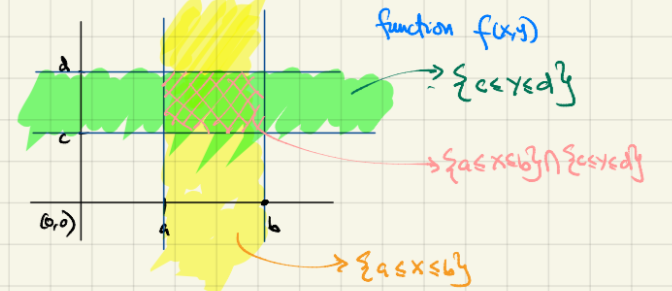
\includegraphics[scale=0.5]{figures/joint_distribution}
\begin{defn}
Given a joint probability density function $f(x,y)$ for X and Y. Then \textbf{Marginal for X}:\begin{align*}
\text{For fixed }x,\\
f_X(x)&=\int_{-\infty}^{\infty}f(x,y)dy
\end{align*}
\textbf{Marginal for Y}:\begin{align*}
\text{For fixed }y,\\
f_Y(y)&=\int_{-\infty}^{\infty}f(x,y)dx
\end{align*}
\textbf{Conditional for X}\begin{align*}
\text{For fixed y,}\\
f_{x|y}(x|y)&=\frac{f(x,y)}{f_Y(y)}
\end{align*}
\textbf{Conditional for Y}
\begin{align*}
\text{For fixed x,}\\
f_{y|x}(y|x)&=\frac{f(x,y)}{f_X(x)}
\end{align*}
Using the \textbf{Multiplication Principle,} we have \begin{align*}
f(x,y)&=f_{x|y}(x|y)\cdot f_Y(y)\text{\quad}\forall x,y\in X\times Y\\
&=f_{y|x}(y|x)\cdot f_X(x)\text{\quad}\forall x,y\in X\times Y
\end{align*} 
\end{defn}
\begin{defn}
We say two random variables X and Y with joint probability mass function $p(x,y)$ or joint probability density function $f(x,y)$ are independent if \begin{align*}
p(x,y)&=p_X(x)\cdot p_Y(y) \text{ }\forall (x,y)\in X\times Y\\
f(x,y)&=f_X(x)\cdot f_Y(y) \text{ }\forall (x,y)\in X\times Y
\end{align*}
\end{defn}
\example Let experiment is as follows: \\
\text{\quad} \textbf{Step 1:} Toss a coin with $P(H)=0.8$ (more generally) $p\in (0,1)$\\
\text{\quad} \textbf{Step 2:} If coin lands H, roll a fair six-sided die. If coin lands T, roll an unfair die with distribution \begin{center}
\begin{tabular}{|l|l|l|l|l|l|}
\hline
1   & 2   & 3   & 4   & 5   & 6   \\ \hline
0.1 & 0.1 & 0.1 & 0.1 & 0.1 & 0.5 \\ \hline
\end{tabular}
\end{center}
Let random variables X, Y defines as below \begin{align*}
X&=\begin{cases}
0&\text{If coin lands T}\\
1&\text{If coin lands H}
\end{cases}\\
Y&=\text{ outcome of the die roll}
\end{align*}
Then, we know that \begin{align*}
X&=\{0,1\}\\
Y&=\{1,2,3,4,5,6\}\\
X\times Y&=\begin{Bmatrix}
(0,1),(0,2),(0,3),(0,4),(0,5),(0,6)\\
(1,1),(1,2),(1,3),(1,4),(1,5),(1,6)\\
\end{Bmatrix}
\end{align*}
The \textbf{Joint Distribution tables:} \begin{center}
\begin{tabular}{|l|l|l|l|l|l|l|}
\hline
 &
  1 &
  2 &
  3 &
  4 &
  5 &
  6 \\ \hline
0 &
  \begin{tabular}[c]{@{}l@{}}$p(0,1)$\\ $0.2\times 0.1$\end{tabular} &
  \begin{tabular}[c]{@{}l@{}}$p(0,2)$\\ $0.2\times 0.1$\end{tabular} &
  \begin{tabular}[c]{@{}l@{}}$p(0,3)$\\ $0.2\times 0.1$\end{tabular} &
  \begin{tabular}[c]{@{}l@{}}$p(0,4)$\\ $0.2\times 0.1$\end{tabular} &
  \begin{tabular}[c]{@{}l@{}}$p(0,5)$\\ $0.2\times 0.1$\end{tabular} &
  \begin{tabular}[c]{@{}l@{}}$p(0,6)$\\ $0.2\times 0.5$\end{tabular} \\ \hline
1 &
  \begin{tabular}[c]{@{}l@{}}$p(1,1)$\\ $0.8\times \frac{1}{6}$\end{tabular} &
  \begin{tabular}[c]{@{}l@{}}$p(1,2)$\\ $0.8\times \frac{1}{6}$\end{tabular} &
  \begin{tabular}[c]{@{}l@{}}$p(1,3)$\\ $0.8\times \frac{1}{6}$\end{tabular} &
  \begin{tabular}[c]{@{}l@{}}$p(1,4)$\\ $0.8\times \frac{1}{6}$\end{tabular} &
  \begin{tabular}[c]{@{}l@{}}$p(1,5)$\\ $0.8\times \frac{1}{6}$\end{tabular} &
  \begin{tabular}[c]{@{}l@{}}$p(1,6)$\\ $0.8\times \frac{1}{6}$\end{tabular} \\ \hline
\end{tabular}
\end{center}
\hfill\\
Now, we can calculate the Marginals and the conditionals.\\
When $x=0,$ \begin{align*}
p_X(0)=\sum_{y=1}^{6}p(0,y)&=0.2\times (0.1+0.1+0.1+0.1+0.1+0.5)\\
&=0.2
\end{align*}
When $x=1,$ \begin{align*}
p_X(1)&=\sum_{y=1}^{6}p(1,y)=0.8\times (\frac{1}{6}\times 6)\\
&=0.8(1)=0.8
\end{align*}
Then, the marginal distribution of X is
\begin{center}
\begin{tabular}{|l|l|l|}
\hline
x        & 0   & 1   \\ \hline
$p_X(x)$ & 0.2 & 0.8 \\ \hline
\end{tabular}
\end{center}
Similarly, we can get Marginal Distribution for Y\begin{center}
\begin{tabular}{|l|l|l|l|l|l|l|}
\hline
y &
  1 &
  2 &
  3 &
  4 &
  5 &
  6 \\ \hline
$p_Y(y)$ &
  \begin{tabular}[c]{@{}l@{}}$0.2\times 0.1+0.9\times \frac{1}{6}=$\\ 0.1533\end{tabular} &
  0.1533 &
  0.1533 &
  0.1533 &
  0.1533 &
  \begin{tabular}[c]{@{}l@{}}$0.2\times 0.5+0.8\times \frac{1}{6}=$\\ 0.233\end{tabular} \\ \hline
\end{tabular}  
\end{center}
\hfill\\
To calculate the conditionals for Y.\\
When $x=0$\begin{align*}
p_{y|x=0}(y|x=0)&=\frac{p(0,y)}{p_X(0)}\\
&=\frac{0.2\times 0.1}{0.2}\\
&=0.1
\end{align*}
Then conditional distribution table for $Y|X=0$ is \begin{center}
\begin{tabular}{|l|l|l|l|l|l|l|}
\hline
y        & 1   & 2   & 3   & 4   & 5   & 6   \\ \hline
$p_{Y|X=0}$ & 0.1 & 0.1 & 0.1 & 0.1 & 0.1 & 0.5 \\ \hline
\end{tabular}
\end{center}
Notice that this is the distribution table of the unfair die.\\
\hfill\\
Similarly, we can calculate when $x=1$.\begin{align*}
p_{y|x}(y|x=1)&=\frac{p(1,y)}{p_X(1)}\\
&=\frac{0.8\times \frac{1}{6}}{0.8}\\
&=\frac{1}{6}
\end{align*}
Then, the conditional distribution table for $Y|X=1$ is\begin{center}
\begin{tabular}{|l|l|l|l|l|l|l|}
\hline
y        & 1   & 2   & 3   & 4   & 5   & 6   \\ \hline
$p_{Y|X=1}$ & $\frac{1}{6}$ & $\frac{1}{6}$ & $\frac{1}{6}$ & $\frac{1}{6}$ & $\frac{1}{6}$ & $\frac{1}{6}$\\ \hline
\end{tabular}
\end{center}
Notice this is the distribution table for the fair die. \\
Intuition: IF we know that $\{X=1\}$ has happened, then we rolled the fair die.\\
\hfill\\
Then we can calculate the condition of X.\\
When $y=1$\begin{align*}
p_{x|y}(x|y=1)&=\frac{p(x,1)}{p_Y(1)}\\
\frac{p(0,1)}{p(0,1)+p(1,1)}&=\frac{0.2\times 0.1}{0.2\times 0.1 +0.8\times \frac{1}{6}}\\
\frac{p(1,1)}{p(0,1)+p(1,1)}&=\frac{0.8\times \frac{1}{6}}{0.2\times 0.1 +0.8\times \frac{1}{6}}\\
\end{align*}
So $Y=1,2\cdots 5$, the conditional of X is
\begin{center}
\begin{tabular}{|l|l|l|}
\hline
x           & 0 & 1 \\ \hline
$p_{x|y=1,2,3,4,5}$ & $\frac{0.2\times 0.1}{0.2\times 0.1 +0.8\times \frac{1}{6}}$  &  $\frac{0.8\times \frac{1}{6}}{0.2\times 0.1 +0.8\times \frac{1}{6}}$ \\ \hline
\end{tabular}
\end{center}
When $Y=6$, the conditional of Y is \begin{center}
\begin{tabular}{|l|l|l|}
\hline
x           & 0 & 1 \\ \hline
$p_{x|y=1}$ & $\frac{0.2\times 0.5}{0.2\times 0.5 +0.8\times \frac{1}{6}}$  &  $\frac{0.8\times \frac{1}{6}}{0.2\times 0.5+0.8\times \frac{1}{6}}$ \\ \hline
\end{tabular}
\end{center}
Observe that all of these calculation are really Bayes Theorem at play.  \\
\hfill\\
Then, we need to see of X and Y are independent.\\
Intuitively, the outcome of the die roll depends on the outcome of the coin toss. To show that, let's take $(x_0,y_0)=(1,6)\in X\times Y$\begin{align*}
p(1,6)&=0.8\times \frac{1}{6}\\
p_X(1)&=0.8\\
p_Y(6)&=0.8\times o.5+0.8\times \frac{1}{6}\\
p_X(1)\cdot p_Y(6)&=0.8(0.2\times 0.5+0.8\times \frac{1}{6})=0.18667\neq 0.1333
\end{align*} 
Therefore, X and Y are not independent.
\section[Distribution of the Sum of Two Independent Random Variables]{\color{DarkOrchid} Distribution of the Sum of Two Independent Random Variables \color{black}}
\begin{thm}
\textbf{Uniqueness of Moment Generating Functions}\\
If X, Y are two random variables with cumulative density functions $F_X(u),F_Y(u)$ respectively and moment generating functions $M_X(t)$ and $M_Y(t)$ respectively.\\
The, \begin{align*}
M_X(t)=M_Y(t)\text{ }\forall t\in (-\delta,\delta)&\implies F_X(u)=F_Y(u)\text{ }\forall u\in \mathbb{R}\\
& \implies X,Y\text{are identically distributed}
\end{align*}
\end{thm}
\begin{thm}
Suppose X, Y are two independent random variables. (i.e $p(x,y)=p_X(x)\cdot p_Y(y)$ $\forall x,y\in \R\times \R$). Then if \begin{align*}
Z&=aX+bY
\end{align*}
then, \begin{align*}
M_Z(t)&=M_{aX+bY}(t)\\
&=M_X(at)\cdot M_Y(bt)
\end{align*}
where $M_X(t),M_Y(t)$ are moment generating functions of X, Y respectively.\\
In particular: if $a=b=1$, if X, Y are independent, \begin{align*}
M_{X+Y}(t)&=M_{X}(t)\cdot M_{Y}(t)
\end{align*}
\end{thm}
\begin{proof}
Suppose X, Y are independent
\begin{align*}
M_{aX+bY}(t)=E(e^{(aX+bY)t}):&=\sum_{(x,y)}e^{(aX+bY)t}\cdot p_X(x)\cdot p_Y(y)\\
&=\sum_{(x,y)}\left( e^{axt}\cdot p_X(x) \right) \left( e^{bxt}\cdot p_Y(y)  \right)\\
&=\left(\sum_{x\in X} e^{axt}\cdot p_X(x) \right) \left( \sum_{y\in Y} e^{bxt}\cdot p_Y(y)  \right)\\
&=M_X(t)\cdot M_Y(t)
\end{align*}
\end{proof}
\begin{thm}
Suppose $X,Y$ are two binomial distribution. \begin{align*}
X&\sim \text{ Binom}(n,p)\\
Y&\sim \text{ Binom}(m,p)\\
\end{align*}
Then if $X,Y$ are independent\begin{align*}
X+Y\sim \text{ Binom}(n+m,p)
\end{align*}
\end{thm}
\begin{proof}
Suppose X, Y are independent. To calculate the moment generating function of $X+Y:$\begin{align*}
M_{X+Y}(t)&=M_{X}(t)\cdot M_{Y}(t)\\
&=\left(p\cdot e^{t}+(1-p) \right)^n\cdot \left(p\cdot e^{t}+(1-p) \right)^{m}\\
&=\left(p\cdot e^{t}+(1-p) \right)^{n+m}
\end{align*}
This is moment generating function of Binom$(n+m,p)$
\end{proof}
\begin{thm}
Suppose $X,Y$ are two binomial distribution. \begin{align*}
X&\sim \text{ Gamma}(\alpha_1,\beta)\\
Y&\sim \text{ Gamma}(\alpha_2,\beta)
\end{align*}
If $X,Y$ are independent \begin{align*}
M_{X+Y}(t)&=M_{X}(t)+M_{Y}(t)\\
&=\left(\frac{1}{1-\beta t} \right)^{\alpha_1}\cdot \left(\frac{1}{1-\beta t} \right)^{\alpha_2}\\
&=\left(\frac{1}{1-\beta t} \right)^{\alpha_1+\alpha_2}
\end{align*}
This is moment generating function of Gamma$(\alpha_1+\alpha_2,\beta)$
\end{thm}
Similarly, can check that the sum of two independent normal distributions is also normal. \\
\note Sum of two independent Poisson distributions is also a Poisson distribution.\\
\hfill\\
\begin{thm}
Suppose \begin{align*}
X\sim  Binom(n,p)\\
Y\sim  Binom(m,p)\\
\end{align*}
X, Y are independent. We say \begin{align*}
Z&=X+Y\sim \text{ Binom}(n+m,p)
\end{align*}
$X|Z\sim $Hypergeo$(N=n+m,M=n,$ sample size $=Z)$
\end{thm}
\begin{proof}
\begin{align*}
p_{X|Z}(x|z)&=\frac{P(X=x \text{ and }Z=z)}{P(Z=z)}\\
&=\frac{P(X=x \text{ and }X+Y=z)}{P(Z=z)}\\
&=\frac{P(X=x,Y=z-x)}{P(Z=z)}\\
&=\frac{\binom{n}{x}\cdot p^{x}(1-p)^{n-x}\cdot \binom{m}{z-x}\cdot p^{z-x}\cdot (1-p)^{m-(z-x)}}{\binom{n+m}{z}\cdot p^z \cdot (1-p)^{n+m-z}}\\
&=\frac{\binom{n}{x}\cdot \binom{m}{z-x}\cdot p^{z-x+x}\cdot (1-p)^{m-z+x+n-x}}{\binom{n+m}{z}\cdot p^z \cdot (1-p)^{n+m-z}}\\
&=\frac{\binom{n}{x}\cdot \binom{m}{z-x}\cdot p^{z}\cdot (1-p)^{m+n-z}}{\binom{n+m}{z}\cdot p^z \cdot (1-p)^{n+m-z}}\\
&=\frac{\binom{n}{x}\cdot \binom{m}{z-x}}{\binom{n+m}{z}}
\end{align*}
This is probability mass function of the Hypergeometric distribution with parameters \begin{align*}
\text{Population Size}&:n+m\\
\#\text{ Successes}&:n\\
\text{Sample Size}&:z 
\end{align*}
\end{proof}
\chapter[Properties of Expectation]{Properties of Expectation}
\section[Covariance]{\color{DarkOrchid}Covariance}
Given two random variables $X,Y$ with joint probability mass function $p(x,y)$ or probability density function $f(x,y)$, and $h:\R\times \R \longrightarrow \R$ is a function.\\
Let $Z=h(x,y)$ is random variable.\\
\hfill\\
Then,\begin{align*}
E(Z)&:=\begin{cases}
\sum_{(x,y)\in X\times Y}h(x,y)\cdot p(x,y) &\text{If both }X,Y \text{ are discrete}\\
\int_{-\infty}^{\infty} \int_{-\infty}^{\infty} h(x,y)f(x,y)&\text{If both }X,Y \text{ are countinous}\\
\end{cases}
\end{align*}
If $h(x,y)=z$\begin{align*}
E(h(x,y))&=\sum_{x,y}h(x,y)p(x,y)\\
&=\sum_{x,y}x\cdot p(x,y)\\
&=\sum_{x}\left(\sum_{y}x\cdot p(x,y)\right)\\
&=\sum_{x}x\cdot \sum_{y} p(x,y)\\
&=\sum_{x}x\cdot p_X(x)&\text{The Expected Value of X with respect to the marginal}\\
&=E(X)
\end{align*}
If $h(x,y)=x^2$, then $E(h(x,y))=E(x^2)$\\
\hfill\\
\begin{defn}
The covariance of $X,Y$ is the expected value of product of the deviations of $X,Y$ from their expected value. To calculate so, let \begin{align*}
h(x,y)&=(x-M_X)(y-M_Y) 
\end{align*}
Then, the covariance is
\begin{align*}
Cov(X,Y)&:=E(h(x,y))\\
&=E((X-M_X)(Y-M_Y))
\end{align*}
\end{defn}
Note that covariance is the multiplication product of deviation of $x$ from $M_X$ and deviation of $y$ from $M_Y$.\\
\hfill\\
In term of applications, the expect value is the measure of location for the values of a random variable. i.e Under reasonable assumption, we would expect most of the values under repeated sampling of a random variable to be close to the expected value of the random variable.\\
We say a value of X is large if it is much larger than $E(X)$. If it is much smaller than $E(X)$ we say it is small.
\hfill\\
To know how the values are distributed about $E(X),$ we need the variance of X. 
\begin{defn}
If large values of X are related to large values of Y. We could have pairs $(x,y)$ such that \begin{align*}
x>>M_X &\text{ and }y>>M_y\\
(x-M_X)>>0 &\text{ and }(y-M_Y)>>0\\
(x-M_X)&(y-M_Y)\geq 0
\end{align*}
This makes a positive contribution to $Cov(X,Y)$
\end{defn}
\begin{defn}
If small values of X are related to small values of Y. We could have pairs $(x,y)$ such that \begin{align*}
x<<M_X &\text{ and }y<<M_y\\
(x-M_X)<<0 &\text{ and }(y-M_Y)<<0\\
(x-M_X)&(y-M_Y)\geq 0
\end{align*}
This $(x,y)$ will make a positive contribution to $Cov(X,Y)$
\end{defn}
\begin{defn}
We will say X and Y are \textbf{positively related} if large values of X are related to large values of Y and small values of X are related to small values of Y. \\
i.e For most pairs $(x,y)$ we will have \begin{align*}
(x-M_X)(y-M_Y)&>>0
\end{align*}
Then, $Cov(X,Y)$ will likely to be positive.
\end{defn}
\begin{defn}
We will say X and Y are \textbf{negatively related} if large values of X are related to small values of Y and small values of X are related to large values of Y. \\
i.e For most pairs $(x,y)$ we will have \begin{align*}
(x-M_X)(y-M_Y)&<<0
\end{align*}
Then, $Cov(X,Y)$ will likely to be negative.
\end{defn}
\begin{defn}
We say the relationship between X and Y is neither positive nor negative if \textbf{i)} large values of X are related to both large values of Y and small values of Y\\
\textbf{ii)} and small values of X are related to both small values of Y and large values of Y\\
\hfill\\
i.e For most pairs $(x,y)$ we have \begin{align*}
x>>M_X &\text{ is related to } \begin{cases}
y>>M_Y\\
\text{or}\\
y<<M_Y
\end{cases}
\end{align*}
and \begin{align*}
x<<M_X &\text{ is related to } \begin{cases}
y>>M_Y\\
\text{or}\\
y<<M_Y
\end{cases}
\end{align*}
Then $Cov(X,Y)\approx 0$ 
\end{defn}
\begin{thm}
When calculating $Cov(X,Y)$, use the formula \begin{align*}
Cov(X,Y)&=E(XY)-E(X)\cdot E(Y)
\end{align*}
\end{thm}
\begin{proof}
\begin{align*}
Cov(X,Y)&=E((X-M_X)(Y-M_Y))\\
&=E(XY-XM_Y-YM_X+M_X\cdot M_Y)\\
&=E(XY)-E(XM_Y)-E(Y\cdot M_X)+E(M_XM_y)\\
&=E(XY)-M_Y\cdot E(X)-M_XE(y)+M_XM_YE(1)\\
&=E(XY)-M_XM_Y-M_XM_Y+M_XM_Y\\
&=E(XY)-E(X)\cdot E(Y)
\end{align*}
\end{proof}
\begin{defn}
\textbf{Correlation coefficient} measure the extent of the relationship between X, Y. Defined as \begin{align*}
Corr(X,Y)=\rho_{x,y}:=\frac{Cov(X,Y)}{\sqrt{V(X)}\cdot \sqrt{V(Y)}}
\end{align*}
\end{defn}
\begin{thm}
The correlation coefficient satisifies the following:\begin{enumerate}
\item $-1\leq Corr(X,Y)\leq 1$
\item $\rho_{x,y}=\pm 1\iff \exists a,b$ such that $Y=aX+b$
\item $\rho_{x,y}=\pm 1 \implies$ perfect linear relationship between X and Y\\
$\rho_{x,y}=0\implies$ no linear relationship between X and Y (but can be other relationship
\end{enumerate}
\end{thm}
\begin{thm}
Suppose $Z=aX+bY$\begin{enumerate}
\item $E(Z)=E(aX+bY)=aE(X)+bE(Y)$
\item $V(Z)=a^2V(X)+b^2V(Y)+2abCov(X,Y)$ 
\end{enumerate}
\end{thm}
\begin{proof}
\begin{align*}
V(Z)&:=E((Z-M_Z)^2)\\
&=E((ax+by-aM_X-bM_Y)^2)\\
&=E((ax-aM_X)+(bY-bM_Y)^2))\\
&=E(a^2(X-M_X)^2+2ab(X-M_X)(Y-M_Y)+b^2(Y-M_Y)^2)\\
&=a^2E((X-M_X)^2)+2abE(X-M_X)(Y-M_Y)+b^2E((Y-M_Y)^2)\\
&=a^2V(X)+b^2V(Y)+2abCov(X,Y)
\end{align*}
\end{proof}
\begin{thm}
If $X_2,X_2,\cdots,X_n$ is a collection of random variable and $a_1,a_2,\cdots a_n\in \R$ i.e \begin{align*}
Z&=a_1X_1+a_2X_2+\cdots +a_nX_n
\end{align*}
then \begin{align*}
V(Z)&=\sum{i=1}^{n}a_i^2V(X_i)+2\sum_{1\leq i<j\leq n}a_ia_jCov(X_i,X_j)
\end{align*}
\end{thm}
\section[Hierarchical Models]{\color{DarkOrchid}Hierarchical Models}
\begin{defn}
We X has a \textbf{mixture distribution} if the distribution of X depends on a quality that is also a distribution.
\end{defn}
\begin{thm}
Let $N\sim Pois(\lambda)$, $Y|N\sim Binom(N,P)$. Then, $Y\sim Pois(\lambda p)$
\end{thm}
\example An insect lays a bunch of eggs. We want to know how many eggs survive.\\ 
Assume \begin{enumerate}[topsep=0pt,itemsep=-1ex,partopsep=1ex,parsep=1ex]
\item P(Survival of a single egg) $=p$
\item Survival of different eggs is independent of each other
\end{enumerate}
\hfill\\
In this setting we are interested in the number of survivals given that there were certain numbers of egg laid.\\
Let $n$ be the number of eggs that the insect has laid is $n$ then $\#$ survival among $n$ eggs $\sim$ Binom$(n,p)$. Then, we can setup the Hierarchy as follow: \\
\text{\qquad} \textbf{Step 1:} Sample $n$ from a distribution.\\
\text{\qquad} \textbf{Step 2:} Use the $n$ from step 1, in Binom$(n,p)$\\
i.e\\
\text{\qquad} \textbf{Step 1:} $N\sim Pois(\lambda)$\\
\text{\qquad} \textbf{Step 2:} $Y|N\sim Binom(N,p)$, where Y $=\#$ surviving eggs\\
\hfill\\
\hfill\\
We want to know the distribution of $Y$. i.e\\\begin{align*}
P(Y=y)&=\sum_{n=0}^{\infty}P(Y=y,N=n)\\
&=\sum_{n=0}^{\infty}P(Y=y|N=n)\cdot P(N=n)\\
&=\sum_{n=0}^{\infty}\binom{n}{y}\cdot p^y \cdot (1-p)^{n-y}\cdot \frac{e^{-\lambda}\lambda^n}{n!}\\
&=p^y \cdot e^{-\lambda}\sum_{n=0}^{\infty}\binom{n}{y}\cdot (1-p)^{n-y}\cdot \frac{\lambda^n}{n!}\\
&=p^y \cdot e^{-\lambda}\sum_{n=0}^{\infty}\frac{n!}{(n-y)!y!}\cdot (1-p)^{n-y}\cdot \frac{\lambda^n}{n!}\\
&=p^y \cdot e^{-\lambda}\sum_{n=0}^{\infty}\frac{1}{(n-y)!y!}\cdot (1-p)^{n-y}\cdot \lambda^n\\
&=\frac{p^y \cdot e^{-\lambda}}{y!}\sum_{n=y}^{\infty}\frac{1}{(n-y)!}\cdot (1-p)^{n-y}\cdot \lambda^n\text{ Since }n<y \text{ }(n-y)!=0
\end{align*}
Then, set $n-y=m$. Then $n=m+y$, $n=y\implies m=0$, and $n=\infty \implies m=\infty$\begin{align*}
&=\frac{p^y \cdot e^{-\lambda}}{y!}\sum_{m=0}^{\infty}\frac{1}{m!}\cdot (1-p)^{m}\cdot \lambda^{m+y}\\
&=\frac{(p\lambda)^y \cdot e^{-\lambda}}{y!}\sum_{m=0}^{\infty}\frac{1}{m!}\cdot (1-p)^{m}\cdot \lambda^{m}\\
&=\frac{(p\lambda)^y \cdot e^{-\lambda}}{y!}\sum_{m=0}^{\infty}\frac{((1-p)\lambda)^{m}}{m!} \text{Power series expansion of }e^{(1-p)\lambda}\\
&=\frac{(p\lambda)^y \cdot e^{-\lambda}}{y!} \cdot e^{\lambda}\cdot e^{-\lambda p}\\
&=\frac{e^{-\lambda p}\cdot (\lambda p)^y}{y!}
\end{align*}
This is the probability mass function of $Pois(\lambda p)$
\section[Conditional Expectation and Variance]{\color{DarkOrchid} Conditional Expectation and Variance}
\begin{thm}
If $X,Y$ are two random variables, then we have the following equality \begin{align*}
E(X|Y)&=E(E(X|Y))
\end{align*}
Where $E(X|Y)$ is a function of Y only.
\end{thm}
\example Recall that given two independent random variables, X and Y where\begin{align*}
X&\sim Binom(n,p)\\
Y&\sim Binom(m,p)\\
\text{Let }Z&=X+Y
\end{align*}
\text{Then, }$X|Z\sim HyperGeo(N=m+n,M=n,\text{ samples zie }=Z)$. Therefore \begin{align*}
E(X|Z)=(\text{ Sample Size }\times \frac{M}{N})&=Z\cdot \frac{n}{m+n}\\
E(E(X|Z))=E\left(Z\cdot \frac{n}{m+n}\right)&=\frac{n}{n+m}\cdot E(Z)\\
&=\frac{n}{n+m}\cdot (n+m)\cdot p\\
&=np=E(X)
\end{align*}
\begin{thm}
\textbf{Conditional Variance}\\
If $X,Y$ are two random variable, then \begin{align*}
V(X)&=E(V(X|Y))+V(E(X|Y))
\end{align*}
\end{thm}
\example Let $X\sim Binom(n,p), Y\sim Binom(m,p)$, where $X,Y$ are independent. Let $Z=X+Y$. Then $X|Z\sim HyperGeo(N=m+n,M=n,\text{ samples zie }=Z)$. Then\\\begin{align*}
E(X|Z)&=\frac{n}{n+m}\cdot Z\\
V(X|Z)&=\frac{n+m-Z}{n+m-1}\cdot Z \cdot \frac{n}{n+m}\cdot \frac{m}{n+m}\\
V(X)&=n\cdot p(1-p)
\end{align*}
Then ,we want to verify \begin{align*}
E(V(X|Z))&=E\left(\frac{n+m-Z}{n+m-1}\cdot Z \cdot \frac{n}{n+m}\cdot \frac{m}{n+m}\right)\\
&=\frac{n}{n+m}\cdot \frac{m}{n+m}\cdot E\left(\frac{n+m-Z}{n+m-1}\cdot Z \right)\\
&=\frac{n}{n+m}\cdot \frac{m}{n+m}\cdot E\left(\frac{nZ+mZ-Z^2}{n+m-1} \right)\\
&=\frac{n}{n+m}\cdot \frac{m}{n+m}\cdot \frac{1}{n+m-1} E\left(nZ+mZ-Z^2 \right)\\
&=\frac{n}{n+m}\cdot \frac{m}{n+m}\cdot \frac{1}{n+m-1} (n(n+m)\cdot p+m(n+m)\cdot p -n(n-1)p^2-np)\\
\end{align*}
\begin{align*}
V(E(X|Z))&=V\left( \frac{n}{n+m}\cdot Z\right)\\
&=\left(\frac{n}{n+m}\right)^2\cdot V(Z)\\
&=\left(\frac{n}{n+m}\right)^2\cdot (n+m)p(1-p)\\
&=\frac{n^2}{n+m} \cdot p\cdot (1-p)
\end{align*}
\chapter[Limit Theorem]{Limit Theorem}
\section[Inequalities for Parameters]{\color{DarkOrchid}Inequalities for Parameters}
We want to arrive at reasonable estimates on certain parameters/probabilities without knowing all the needed information.\\
\hfill\\
\example Given two random variables $X,Y$. Say we want to know $E(XY)$, then we need the joint probability mass density/probability density function, so that we can calculate \begin{align*}
E(XY)&=\sum_{x,y}xy\cdot p(x,y)
\end{align*}
To be able to calculate $p(x,y)$, we need the marginals $p_X(x)$, $p_Y(y)$ for all $x,y$ and conditionals $p_{X|Y}(X|Y)$, $p_{Y|X}(y|x)$. So that we can use the multiplication principle.\\
\hfill\\
\textbf{1. Holders Inequality}\\
\begin{thm}Given two random variables $X,Y$ and $p,q>1$ such that \begin{align*}
\frac{1}{p}+\frac{1}{q}&=1
\end{align*}
then \begin{align*}
|E(XY)|&\leq E(|X|^p)^{\frac{1}{p}} \cdot E(|Y|^q)^{\frac{1}{q}}
\end{align*}
\end{thm}
\note \begin{enumerate}
\item Calculation of $E(XY)$ needs both the conditionals and marginals for X and Y
\item Calculation of $E(|X|^p)$ needs marginal of X. Calculation of $E(|Y|^q)$ needs marginal of $X$.
\end{enumerate}
\textbf{Application of Holder:} Cauchy-Schwartz Inequality take $p=q=2$, so that $\frac{1}{p}+\frac{1}{q}=\frac{1}{2}+\frac{1}{2}=1$\\
In this setting \begin{align*}
|E(XY)|&\leq E(|X|^2)^{\frac{1}{2}}\cdot E(|Y|^2)^{\frac{1}{2}}
\end{align*}
\textbf{Application of Cauchy-Schwartz:} Given $X,Y$ with expected value $M_X,M_Y$ respectively. Then, \begin{align*}
R&=(X-M_X)\\
S&=(Y-M_Y)
\end{align*}
Now apply \textbf{Cauchy Schwarz} to $R,S$ to get \begin{align*}
|E(R\cdot S)|&\leq E(|R|^2)^{\frac{1}{2}} \cdot E(|S|^2)^{\frac{1}{2}}\\
|E((X-M_X)(Y-M_X))|&\leq E((X-M_X))\cdot E((Y-M_Y)^2)^{\frac{1}{2}}\\
|Cpv(X,Y)|&\leq \sqrt{V(X)}\cdot \sqrt{V(X)}
\end{align*}
This is the \textbf{Covariance Inequality}\\
\note If $V(X),V(Y)>0$ (ie $\neq 0$). We get \begin{align*}
\frac{|Cov(X,Y)|}{\sqrt{V(X)}\cdot \sqrt{V(Y)}}&\leq 1
\end{align*}
Using covariance identity we have shown that \begin{align*}
|Corr(X,Y)|&\leq 1
\end{align*}
\example Suppose $X,Y$ have the following table \begin{center}
\begin{tabular}{|l|l|l|l|l|l|l|}
\hline
 &
  1 &
  2 &
  3 &
  4 &
  5 &
  6 \\ \hline
0 &
  \begin{tabular}[c]{@{}l@{}}$p(0,1)$\\ $0.2\times 0.1$\end{tabular} &
  \begin{tabular}[c]{@{}l@{}}$p(0,2)$\\ $0.2\times 0.1$\end{tabular} &
  \begin{tabular}[c]{@{}l@{}}$p(0,3)$\\ $0.2\times 0.1$\end{tabular} &
  \begin{tabular}[c]{@{}l@{}}$p(0,4)$\\ $0.2\times 0.1$\end{tabular} &
  \begin{tabular}[c]{@{}l@{}}$p(0,5)$\\ $0.2\times 0.1$\end{tabular} &
  \begin{tabular}[c]{@{}l@{}}$p(0,6)$\\ $0.2\times 0.5$\end{tabular} \\ \hline
1 &
  \begin{tabular}[c]{@{}l@{}}$p(1,1)$\\ $0.8\times \frac{1}{6}$\end{tabular} &
  \begin{tabular}[c]{@{}l@{}}$p(1,2)$\\ $0.8\times \frac{1}{6}$\end{tabular} &
  \begin{tabular}[c]{@{}l@{}}$p(1,3)$\\ $0.8\times \frac{1}{6}$\end{tabular} &
  \begin{tabular}[c]{@{}l@{}}$p(1,4)$\\ $0.8\times \frac{1}{6}$\end{tabular} &
  \begin{tabular}[c]{@{}l@{}}$p(1,5)$\\ $0.8\times \frac{1}{6}$\end{tabular} &
  \begin{tabular}[c]{@{}l@{}}$p(1,6)$\\ $0.8\times \frac{1}{6}$\end{tabular} \\ \hline
\end{tabular}
\end{center}
Marginal distribution of X is
\begin{center}
\begin{tabular}{|l|l|l|}
\hline
x        & 0   & 1   \\ \hline
$p_X(x)$ & 0.2 & 0.8 \\ \hline
\end{tabular}
\end{center}
Marginal Distribution for Y\begin{center}
\begin{tabular}{|l|l|l|l|l|l|l|}
\hline
y &
  1 &
  2 &
  3 &
  4 &
  5 &
  6 \\ \hline
$p_Y(y)$ &
  \begin{tabular}[c]{@{}l@{}}$0.2\times 0.1+0.9\times \frac{1}{6}=$\\ 0.1533\end{tabular} &
  0.1533 &
  0.1533 &
  0.1533 &
  0.1533 &
  \begin{tabular}[c]{@{}l@{}}$0.2\times 0.5+0.8\times \frac{1}{6}=$\\ 0.233\end{tabular} \\ \hline
\end{tabular}  
\end{center}
Then, we calculate \begin{align*}
E(XY)&=\sum_{x,y}xy\cdot p(x,y)\\
&=\sum_{y=1}^{6}1\cdot y \cdot p(1,y) \text{ }x=0\text{ does not contribute}\\
&=1\cdot 0.8\cdot \frac{1}{6}+2\cdot 0.8 \cdot \frac{1}{6} +\cdots +6\cdot 8\cdot \frac{1}{6}\\
&=\frac{0.8}{6}\cdot (1+2+3+\cdot +6)\\
&=\frac{0.8}{6}\cdot \frac{6\cdot 7}{2}\\
&=0.4\cdot 7=2.8
\end{align*}
Now: Suppose $p=q=2$, we than calculate $E(X^2)$ and $E(Y^2)$\begin{align*}
E(X^2)&=\sum_{x}x^2\cdot p_X(x)\\
&=1\times 0.8=0.8
\end{align*}\begin{align*}
E(Y^2)&=\sum_{y}y^2\cdot p_Y(y)\\
&=1^2\left(0.2\times 0.1+0.8\times \frac{1}{6}\right)+\cdots \\
&+6^2\left(0.2 \times 0.5+0.8\times \frac{1}{6}\right)\\
&=16.833
\end{align*}
\begin{align*}
2.8&\leq \sqrt{0.8}\cdot \sqrt{16.833}=3.66965
\end{align*}
So Holder's identity is true!\\
\hfill\\
\example Suppose \begin{align*}
X&\sim Binom(n=10,p=0.2)\\
Y&\sim Gamma(\alpha=2, \beta=3)
\end{align*}
Now, we want to estimate $|E(XY)|$. \\
\hfill\\
Let's take $p=1=2$. Then by Holder's Inequality. \begin{align*}
E(XY)&\leq (E(X^2))^{\frac{1}{2}}\cdot (E(Y^2))^{\frac{1}{2}}
\end{align*}
Then \begin{align*}
E(X^2)=V(X)+E(X)^2\\
&=n\cdot p(1-p)+(np)2\\
&=10\times 0.2\times 0.8+(10\times 0.2)^2\\
&=1.6+4=5.6
\end{align*}\begin{align*}
E(Y^2)&=V(Y)+E(Y)^2\\
&=\alpha \cdot \beta^2+(\alpha \beta)^2\\
&=2\times 9 +(2\times 3)^2\\
&=18+36 =54
\end{align*}
Then, \begin{align*}
|E(XY)|&\leq \sqrt{5.6}\times \sqrt{54}\\
|Cov(X,Y)|&\leq \sqrt{V(X)}\cdot \sqrt{V(Y)}\\
&\leq \sqrt{1.6}\cdot\sqrt{18}\\
&\leq 5.3665
\end{align*}
\textbf{2. Minkowski's Inequality}\\
\begin{thm}
Suppose $X,Y$ are random variable and $p\in [1,\infty]$, then \begin{align*}
E(|X+Y|^p)^{\frac{1}{p}}&\leq E(|X|^p)^{\frac{1}{p}}+E(|Y|^p)^{\frac{1}{p}}
\end{align*}
\end{thm}
\exercise Suppose \begin{align*}
X&\sim Binom(n=10,p=0.2)\\
Y&\sim Gamma(\alpha =2,\beta =3) 
\end{align*}
We want a bound for \begin{align*}
\left(E(|X+Y|^3)\right)^{\frac{1}{3}}&\leq E(X^3)^{\frac{1}{3}}+E(Y^3)^{\frac{1}{2}}
\end{align*}
We want to using moment generating functions of X and Y to get there. 
\section[Inequalities For Probabilities]{Inequalities For Probabilities}
\textbf{1. Markou's Inequality}\\
\begin{thm}
If X is a positive random variable (i.e support is $\geq 0$). For any $a>0$, we have \begin{align*}
E(X\geq a)&\leq \frac{E(X)}{a}
\end{align*}
\end{thm}
\begin{center}
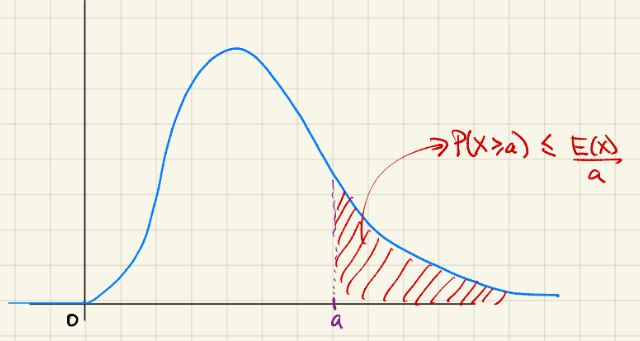
\includegraphics[scale=0.5]{figures/graph1.1}
\end{center}
\note The only number need to estimate $P(X\geq a)$ using Markov's inequality is $E(X)$. As a result the bounds will be pretty coarse (sometime useless)\\
\hfill\\
\textbf{1. Chebychev's Inequality}\\
\begin{thm}
If X is any random variable with $E(X)=M$ and $V(X)=\sigma^2<\infty$, then for any $k\leq 0,$\begin{align*}
P(|X-M|\geq k)&\leq \frac{\sigma^2}{k^2} 
\end{align*}
\end{thm}
\begin{proof}
Notice $(X-M_X)^2$ is a positive random variables.\\
Using Markous, we have \begin{align*}
P(|X-M|\geq k)&=P((X-M)^2\geq k^2)\\
&\leq \frac{E((X-M)^2)}{k^2}\\
&=\frac{V(X)}{k^2}\\
&=\frac{\sigma^2}{k^2}
\end{align*}
\end{proof}
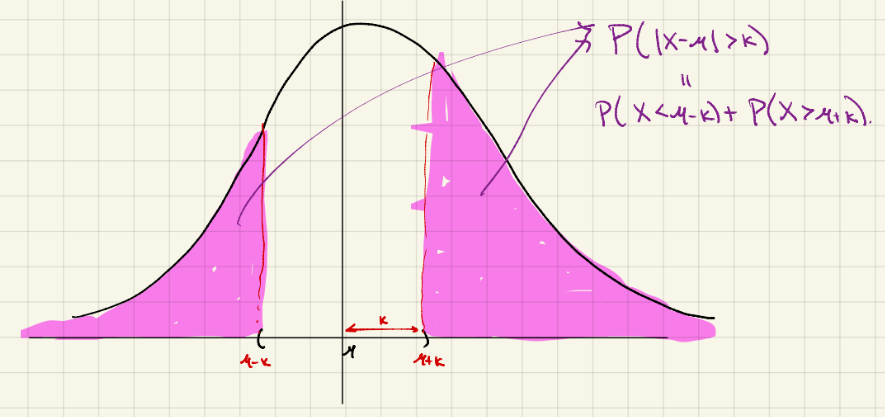
\includegraphics[scale=0.5]{figures/chebycheus}
\chapter[Random Sample and Statistic]{Random Sample and Statistic}
Given a population, we can uses a random variable to analyze the information about this characteristic remains fixed once the population of interest is identified.\\
However, calculating the number is usually not possible due to the following \\
 \begin{enumerate}[topsep=0pt,itemsep=-1ex,partopsep=1ex,parsep=1ex]
\item The population might be to large or inaccessible.
\item Not all individuals in the population might be accessible
\item Computational/physical resources might not exist
\end{enumerate}
\hfill\\
Then, we can have a sample that is typically much smaller than the size of the population\begin{center}
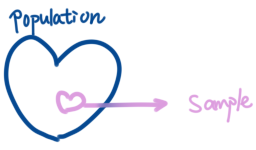
\includegraphics[scale=0.6]{figures/sample_popilation}
\end{center}
And the information obtained using a sample is called a statistic, which has the following properties \begin{enumerate}[topsep=0pt,itemsep=-1ex,partopsep=1ex,parsep=1ex]
\item The value of a statistic depends on much smaller set of individuals obtained from the population, which is easier to calculate
\item The value of the statistic will depend on the sample. Therefore we have to be careful about how we interpret this value 
\end{enumerate}
\hfill\\
\begin{defn}
A \textbf{random sample} of size n is a collection of n independent and identical distributed random variables.\\
More precisely: We say $\{X_1,X_2,\cdots ,X_n\}$ is a random sample of size n if \begin{enumerate}
\item $X_1,X_2,\cdots,X_n$ are identical to a fixed common distributed say X. \\
 i.e $X_i\sim X$ $\forall i=1,2,\cdots,n$
\item $X_1,X_2,X_3,\cdots,X_n$ are independent. \\
i.e If $P_X(x)$ is the probability mass of X (the common distribution), then \begin{align*}
p\left(X_1,X_2,\cdots,X_n\right)&=p_X(X_1)\cdot p_X(X_2) \cdots p_X(X_n)
\end{align*}
\end{enumerate}
\end{defn}
\note The common distribution for the $X_i's$, i.e X is called the population distribution.\\ 
\note If $x$ is the values of X, then the joint sample space for $X_1,X_2,\cdots,X_n$ is \begin{align*}
X_1\times X_2\times \cdots \times X_n&=x^n
\end{align*}
\example Suppose the population is the set \begin{align*}
\{1,2,3,4,5\}&\longrightarrow \text{population}
\end{align*}
Choose a random sample of size 3. \begin{align*}
\{N_1,N_2,N_3\}
\end{align*}
$N_i$ is sample a number from the population. If $N_1$ and $N_2$ have to be independent, we need to sample replacement. Then, the joint sample space for $N_1,N_2,N_3$ is \begin{align*}
\begin{Bmatrix}
(1,1,1),(1,2,1),(1,1,2)\cdots\\
\cdots (5,5,3),(5,5,4),(5,5,5)
\end{Bmatrix}
\end{align*}
which is all possible samples of size 3 from the population.\\
\note \begin{enumerate}[topsep=0pt,itemsep=-1ex,partopsep=1ex,parsep=1ex]
\item The random sample is a collection of random variables.
\item Sample data is one possible entry in the joint sample space of a random sample.
\end{enumerate}
\begin{defn}
A statistic is a quantity that is calculated only using a random sample.\\
i.e: Given a random sample $\{X_1,X_2,\cdots,X_n\}$, a statistic is a function of $X_1,X_2,\cdots,X_n$\\
i.e: $\hat{\theta}$ is a statistic, then $\hat{\theta}=$function$(X_1,\cdots,X_n)$
\end{defn}
\note The value of a statistic change everytime we sample the population.\\
i.e Statistic is s a random variable. This is what we interested in the distribution of this random variable. This is sampling distribution of the statistic.\\
\hfill\\
\begin{defn}
Given a population $\{1,2,3,\cdots,n\}$, and random sample $\{N_1,N_2,\cdots,N_i\}$. Then, they will have the statistics as follow:\\
The \textbf{sample mean} is \begin{align*}
\overline{X}&=\frac{N_1+N_2+\cdots+N_i}{i}
\end{align*}
The \textbf{sample total} is \begin{align*}
T_o&=N_1+N_2+\cdots +N_i
\end{align*}
The \textbf{sample max} is \begin{align*}
Max&(N_1,N_2,\cdots, N_i)
\end{align*}
The \textbf{sample median} is \begin{align*}
\widetilde{X}&=Median(N_1,N_2,\cdots,N_i)
\end{align*}
\end{defn}
\note A statistic $\hat{\theta}$ is a function defined on the joint sample space $X^n$ of $X_1,\cdots,X_n$.i.e\begin{align*}
\hat{\theta}:X^n&\longrightarrow \mathbb{R}
\end{align*}
\note Value of $\hat{\theta}$ depends on the sample distribution. It  is a random variable with sample space $X^n$. \\
\hfill\\
Given a statistic, calculate its sampling distribution.\\
\section[Brute Force]{\color{DarkOrchid}Brute Force}
Given a a statistic, we can explictily list out $X^n$ and the values of the statistic, and then use the distribution of X and the independence of $X_1,X_2,\cdots,X_n$ to get the distribution of the statistic explicitly.\\
\hfill\\
\textbf{Advantages: }The process is easy and explicit and we get the exact distribution\\
\textbf{Disadvantages: } Even for small values of n, and small population size, the time and space needed to list out $X^n$ might be intractable. \\
\hfill\\
\example Given a population $\{1,2,3,4,5\}$ with population distribution \begin{center}
\begin{tabular}{|l|l|l|l|l|l|}
\hline
x        & 1             & 2             & 3             & 4             & 5             \\ \hline
$p_X(x)$ & $\frac{1}{5}$ & $\frac{1}{5}$ & $\frac{1}{5}$ & $\frac{1}{5}$ & $\frac{1}{5}$ \\ \hline
\end{tabular} $\sim X$
\end{center}
(i) Let sample size $=1$. The statistic sample mean is \begin{align*}
\overline{X}&=\frac{X_1}{1}=X_1
\end{align*}
And the values of $\overline{X}=\overline{x}=\{1,2,3,4,5\}$. And then the sampling distribution of $\overline{X}$ is \begin{center}
\begin{tabular}{|l|l|l|l|l|l|}
\hline
x        & 1             & 2             & 3             & 4             & 5             \\ \hline
$p_X(x)$ & $\frac{1}{5}$ & $\frac{1}{5}$ & $\frac{1}{5}$ & $\frac{1}{5}$ & $\frac{1}{5}$ \\ \hline
\end{tabular}
\end{center}
(ii) Suppose $n=2,$ $\overline{X}=\frac{X_1+X_2}{2}$. The joint sample space is \begin{align*}
\begin{Bmatrix}
(1,1),(1,2),(1,3),(1,4),(1,5)\\
(2,1),(2,2),(2,3),(2,4),(2,5)\\
\vdots\\
(5,1),(5,2),(5,3),(5,4),(5,5)
\end{Bmatrix}
\end{align*}
The value of $\overline{X}=\overline{x}=\{1,1.5,2,2.5,3,3.5,4,4.5,5,5.5,6\}$. The distribution is \begin{center}
\begin{tabular}{|l|l|l|l|l|l|l|l|l|l|}
\hline
$\overline{x}$ & 1              & 1.5            & 2              & 2.5            & 3              & 3.5            & 4              & 4.5            & 5              \\ \hline
$p_X(x)$       & $\frac{1}{25}$ & $\frac{2}{25}$ & $\frac{3}{25}$ & $\frac{4}{25}$ & $\frac{5}{25}$ & $\frac{4}{25}$ & $\frac{3}{25}$ & $\frac{2}{25}$ & $\frac{1}{25}$ \\ \hline
\end{tabular}
\end{center}
\begin{center}
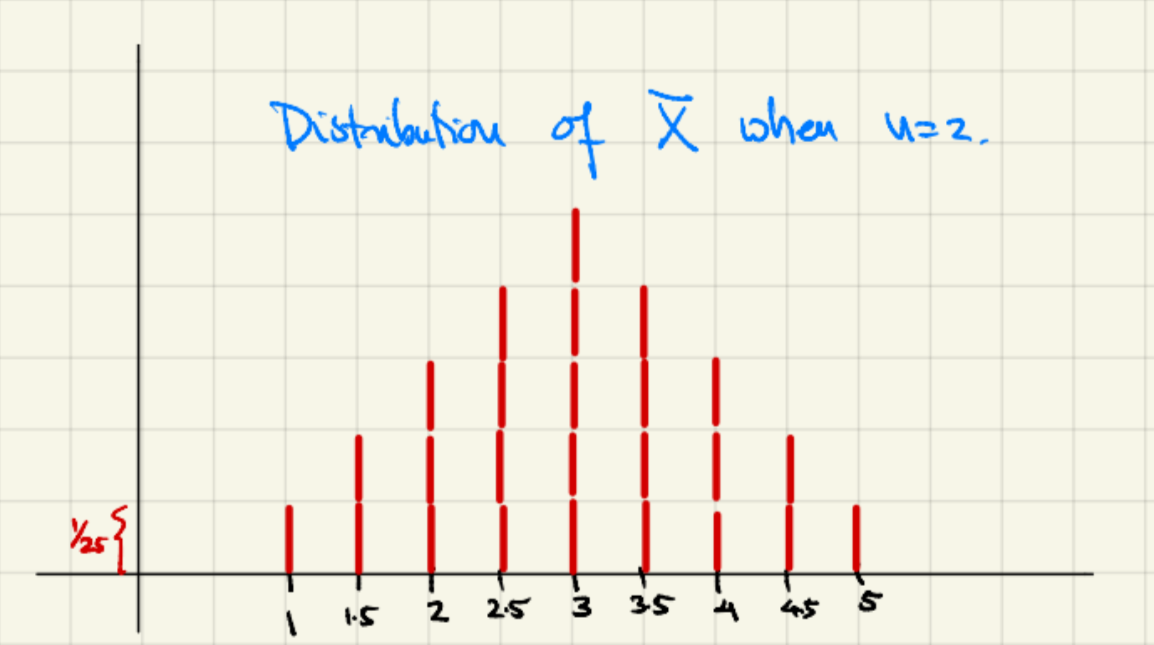
\includegraphics[scale=0.3]{figures/graph_distribution}
\end{center}
\section[Using Moment Generating Function]{\color{DarkOrchid}Using Moment Generating Function}
\begin{thm}
\textbf{Uniqueness of Moment Generating Functions}\\
X and Y have identical moment generating functions if and only if X and Y have identical distribution.
\end{thm}
\begin{thm}
\textbf{Moment Generating Functions of Linear Combination.}\\
If $X_1,X_2,\cdots,X_n$ are mutually independent random variables with moment generating functions $M_{X_1}(t),\cdots,M_{X_n}(t)$ and \begin{align*}
Y&=a_1X_1+a_2X_2+\cdots +a_nX_n
\end{align*}
then \begin{align*}
M_Y(t)&=\prod_{i=1}^{n}M_{X_i}(a_it)
\end{align*}
\end{thm}
\begin{proof}
\begin{align*}
M_Y(t)&=E(e^{Yt})=E(e^{\sum a_ix_it})\\
&=\sum_{x\in X^n}e^{a_1x_1t}\cdot e^{a_2x_2t}\cdot \cdots e^{a_nx_nt}\cdot p_{x_1,\cdots,x_n}\\
&=\sum_{x_1}\sum_{x_2}\cdots \sum_{x_n}e^{a_1x_1t}\cdot e^{a_2x_2t}\cdot \cdots e^{a_nx_nt}\cdot p_X(x_1)\cdots p_X(x_n)\\
&=\left(\sum_{x_1}e^{a_1x_1t}p_X(x_2) \right)\left(\sum_{x_2}e^{a_2x_2t}p_X(x_2)  \right)\cdots \left(\sum_{x_n}e^{a_nx_nt}p_X(x_n) \right)\\
&=M_{X_1}(a_1t)\cdot \cdots M_{X_n}(a_2t)
\end{align*}
\end{proof}
\begin{corT}
If $Y=aX+b$ and $M_X(t)$ is the moment generating functions of X, then \begin{align*}
M_Y(t)&=e^{bt}\cdot M_X(at)
\end{align*} 
\end{corT}
\begin{corT}
If $X_1,X_2,\cdots,X_n$ are mutually independent random variables with moment generating functions $M_{X_1}(t),\cdots,M_{X_n}(t)$ and \begin{align*}
Y_i&=a_iX_i+b_i\\
\text{and }Y&=\sum_{i=1}^{n}Y_i
\end{align*}
then \begin{align*}
M_Y(t)&=e^{\sum_{i=1}^nb_it}\cdot \prod_{i=1}^{n}M_{X_i}(a_it)
\end{align*}
\end{corT}
\textbf{Applications of theorem to calculate sampling distribution of statistics}:\\
\text{\qquad} Suppose $\{X_1,X_2,\cdots,X_n\}$ is a random sample from  population with distribution X. X has moment generating function $M_X(t),$ and $Y=a_1X_1+\cdots +a_nX_n$.\\
Then, \begin{align*}
M_{Y}(t)&=\prod_{i=1}^{n}M_{X_i}(a_it)\\
&=\prod_{i=1}^{n}M_{X}(a_it)&\text{Since they are identically distributed to X}
\end{align*}
i) the sample total. If \begin{align*}
T_o&:=\text{Sample\_Total}
&:=X_1+X_2+\cdots +X_n
\end{align*}
then \begin{align*}
M_{T_o}(t)&=\prod_{i=1}^{n}M_X(t)\\
&=\left( M_X(t)\right)^n
\end{align*}
ii) If \begin{align*}
\overline{X}&:=\text{Sample\_Mean}\\
&:=\frac{X_1+\cdots +X_n}{n}=\frac{T_o}{n}
\end{align*}
then \begin{align*}
M_{\overline{X}}(t)&=\prod_{i=1}^{n}M_{X}\left( \frac{t}{n}\right)\\
&=M_{T_o}\left( \frac{t}{n}\right)\\
&=\left( M_{X}\left(\frac{t}{n} \right)\right)^n
\end{align*}
\example $X\sim $Bernoulli distribution with parameter p. And $\{X_1,\cdots,X_n\}$ is a random sample from X. Recall that \begin{align*}
M_{X}(t)&=pe^{t}+(1-p)
\end{align*}
Then \begin{align*}
M_{T_o}(t)&=\left(M_X(t) \right)^n\\
&=\left(pe^t+(1-p) \right)^n
\end{align*}
This is the moment generating function of Binom(n,p). Then sample total for a random sample from Bernoulli(p) has the binomial distribution.\begin{align*}
M_{\overline{X}}(t)&=\left( M_X\left(\frac{t}{n} \right)\right)^n\\
&=\left( pe^{\frac{t}{n}} +(1-p)\right)^n
\end{align*}
We cannot use the moment generating function of $\overline{X}$ to get its sampling distribution.\\
\hfill\\
\example $X\sim$Binom(n,p), and sample size $=m$. Recall that \begin{align*}
M_{X}(t)&=(pe^t+(1-p))^n
\end{align*}
Then, \begin{align*}
M_{T_o}(t)&=(M_X(t))^n=((pe^t+(1-p)^n)^m\\
&=(pe^t+(1-p)^{nm}
\end{align*}
This is the moment generating function of Binom($nm$, p)\\
\hfill\\
\example $X\sim$N($\mu$,$\sigma^2$), $M_X(t)=e^{\mu t+\frac{\sigma^2 t^2}{2}}$. Then \begin{align*}
M_{t_o}&=\left( M_X(t)\right)^n=\left( e^{\mu t+\frac{\sigma^2 t^2}{2}}\right)^n\\
&=e^{n\mu t+\frac{n\sigma^2 t^2}{2}}\\
&=e^{n\mu t+\frac{(\sqrt{n}\sigma)^2 t^2}{2}}
\end{align*}
This is moment generating functions of $N$(mean $=n\mu$, Variance $=n\sigma^2$).\\
Also: \begin{align*}
M_{\overline{X}}(t)&=\left( M_X\left(\frac{t}{n} \right)\right)^n\\
&=\left(e^{\frac{\mu t}{n}+\frac{\sigma^2 \left(\frac{r}{n}\right)^2}{2}} \right)^n
\end{align*}
This is the moment generating function of $N\left(\mu, \frac{\sigma^2}{n}\right)$\\
\hfill\\
\example $X\sim Gamma(\alpha,\beta)$, $M_X(t)= \left( \frac{1}{1-\beta t}\right)^{\alpha}$.\\
Then \begin{align*}
M_{t_o}&=\left( M_X(t)\right)^n=\left(\left( \frac{1}{1-\beta t}\right)^{\alpha} \right)^n\\
&=\left( \frac{1}{1-\beta t}\right)^{\alpha n} 
\end{align*}
This is $Gamma(n\alpha, \beta)$.\\
Also: \begin{align*}
M_{\overline{X}}(t)&=\left( \frac{1}{1-\frac{\beta t}{n}}\right)^{\alpha n} 
\end{align*}
This is not clear about distribution.\\
\hfill\\
This is limits the applicability to simple statistic that are linear combinations.
\section[Order Statistic]{\color{DarkOrchid}Order Statistic}
\begin{defn}
Given a random sample $\{X_1,X_2,\cdot,X_n\}$. The \textbf{ith order statistic is defined as}:\begin{align*}
X_{(j)}&=j^{\text{th}} \text{ smallest number in the random sample}
\end{align*}
\note $X_{(j)}$ is defined for $j=1,2,\cdots, n$\\
\text{\qquad} $X_{(j)}=1$st smallest number 
\end{defn}
We can use order statistic to calculate the sample median, sample range.\\
\begin{align*}
\text{Sample Median}&=\begin{cases}
X_{\frac{n+1}{2}}&n\in 2\Z+1\\
\frac{X_{\frac{n}{2}}+X_{\frac{n+1}{2}}}{2}&n\in 2\Z
\end{cases}
\end{align*}
\begin{thm}
\textbf{Order Statistics for a Discrete Distribution:}\\
Suppose $X$ has values $x=\{x_1,x_2.x_3,\cdots,x_n\}$ arranged in ascending order and the distribution of $X$ is\begin{center}
\begin{tabular}{|l|l|l|l|l|}
\hline
$x$      & $x_1$ & $x_2$ & $\cdots$ & $x_n$ \\ \hline
$p_X(x)$ & $p_1$ & $p_2$ & $\cdots$ & $p_n$ \\ \hline
\end{tabular}
\end{center}
where $\sum p_i=1$. Nowe we define $P_i$ as follows\begin{align*}
p_1&=p_1\\
p_2&=p_1+p_2\\
\cdots & \cdots\\
p_n&=p_1+p_2+\cdots +p_n
\end{align*}
Set $\{X_{(1)}, X_{(2)},\cdots, X_{(n)}\}$ be the order statistic for a random sample of size n. Then, if $X_{(j)}$ is $j^{\text{th}}$ order statistic.
\begin{enumerate}
\item \begin{align*}
 P(X_{(j)}\leq x_i)&=\sum_{k=j}^n \binom nk p_i^k\cdot (1-p_i)^{n-k}
\end{align*} 
\item \begin{align*}
P(X_{(j)}=x_i)&=P(X_{(j)}\leq x_i)-P(X_{(j)}\leq x_{i-1})\\
&=\sum_{k=j}^n \left(\binom nk \left(p_i^k(1-p_i)^{n-l}-p_{i-1}^k(1-p_{i-1})^{n-k} \right) \right)
\end{align*}
\end{enumerate}
\end{thm}
\hfill\\
\begin{proof}
\hfill\\
If we want to calculate $P(X_{(j)}\leq x_i)$, we can convert the problem into a problem with a familiar underlying distribution.\begin{center}
The event of interest $\longrightarrow$ $\{X_{(j)}\leq x_i\}$\\
\end{center}
We can then define a new random variables \begin{align*}
Y&=\#\text{}X_{k}\text{ in the sample that are less or equal to }x_i\\
\{Y\geq j\}&=\{j \text{ or more entries} \text{ that are less than or equal to }x_i \}
\end{align*}
Note that $\{X_{j}\leq x_i\}$ is the event that jth smallest entry is less zthan or equal to $x_i$, which is same as the number of entries that less than or equal to $x_i$ is greater than or equal to j, which is $\{Y\geq j\}$. Therefore, \begin{align*}
P(X_{(j)}\leq x_i)&= P(Y\geq j)
\end{align*}
Now we want to calculate the distribution of Y. Let arbitary entries in X be $x_k$ \begin{align*}
P(Y=r)&=P(\#\text{ }x_k\text{ less or equal to }x_i \text{ is exactly equal to }r  )
\end{align*}
Suppose $\{X_k\leq x_i \}$ to be a success, then $
P(X_k\leq x_i)$ is the same for all $k=1,2,...,n$\begin{center}
Y $\sim$ Counting the number of successes in $n$ trials where $P(S)=P(x_k\leq x_i)=p$.
\end{center}
Therefore \begin{align*}
P(Y=r)&=\binom nr p^r \cdot (1-p)^{n-r}
\end{align*}
So now we want to find the p. \begin{align*}
P(S)&= P(X_k\leq x_i)\\
&=P(X_k=x_1)+P(X_k=x_2)+\cdots+P(X_k=x_i)\\
&=p_1+p_2+\cdots+p_i\\
&=P_i
\end{align*}
Then\begin{align*}
P(Y=r)=\binom nr P_i^r \cdot (1-P_i)^{n-r}
\end{align*}
Finally, \begin{align*}
P(X_{j}\leq x_i)&=P(Y\geq k)\\
&=P(Y=j)+P(Y=j+1)+\cdots + P(Y=n)\\
&=\sum_{k=j}^n P(Y=k)\\
&=\sum_{k=j}^n \binom nk \cdot P_i^k \cdot (1-P_i)^{n-k}
\end{align*}
Now \begin{align*}
P(X_{j}=x_i)&=P(X_{(j)}\leq x_i)-P(X_{(j)}\leq x_{i-1})\\
&=\sum_{k=j}^{n}\binom nk \left( P_i^{k} (1-P_i)^{n-k}-P_{i-1}^k(1-P_{i-1})^{n-k}\right)
\end{align*}
\end{proof}
\example X has distribution \begin{center}
\begin{tabular}{|l|l|l|l|l|}
\hline
x        & 2   & 5   & 8   & 10  \\ \hline
$p_X(x)$ & 0.1 & 0.4 & 0.2 & 0.3 \\ \hline
\end{tabular}
\end{center}
Say $n=4$, the \begin{align*}
X_{(1)}((2,2,5,8))&=2\\
X_{(1)}((5,2,8,5))&=X_{(1)}((2,2,5,8))=2\\
X_{(3)}((2,5,2,8))&=X_{(3)}((2,2,5,8))=5
\end{align*}
For small sample size $n,$ it is possible to calculate the distribution of the order statistic explicitly. However, calculating the distribution of $X_{(j)}$ when sample size is large is intractable problem. But we c.\\
\hfill\\
\example Toss a coin 7 times. i.e $X\sim Bernoulli(p)$ with a random sample of size 7. We want to calculate the distribution of $X_{(7)}$, the sample max.\\
Note value of $X_{(7)}=\{0,1\}$. We want to calculate \begin{align*}
P(X_{(7)})&=0\\
&=P(\text{7th smallest entry is 0})\\
&=P(\text{All entries in the sample data are 0})\\
&=(1-p)^{7}
\end{align*}
So the distribution table for $X_{(7)}$ is \begin{center}
\begin{tabular}{|l|l|l|}
\hline
x                      & 0         & 1           \\ \hline
$p_{X_{(7)}}(x)$ & $(1-p)^7$ & $1-(1-p)^7$ \\ \hline
\end{tabular}
\end{center}
Now, let's calculate the distribution of $X_{(4)}$. This also sample median.\\
First, let's calculate \begin{align*}
P(X_{(4)}=0)&=P(\text{At least 4 zeroes in 7 tosses})\\
&=P(\text{At most 3 ones in 7 tosses})\\
&=\binom 74 (1-p)^4\cdot p^3+\binom 75 (1-p)^5\cdot p^2+\binom 76 (1-p)^6\cdot p+\binom 77 (1-p)^7
\end{align*}
Setting $q=\binom 74 (1-p)^4\cdot p^3+\binom 75 (1-p)^5\cdot p^2+\binom 76 (1-p)^6\cdot p+\binom 77 (1-p)^7$. The distribution of $X_{(4)}$ is\begin{center}
\begin{tabular}{|l|l|l|}
\hline
x                & 0   & 1     \\ \hline
$p_{X_{(4)}}(x)$ & $q$ & $1-q$ \\ \hline
\end{tabular}
\end{center}
\end{document}